\documentclass[11pt]{article}
\usepackage[T1]{fontenc}
\usepackage[utf8]{inputenc}
\usepackage{lmodern}
\usepackage{amsmath}
\usepackage[margin=2.2cm]{geometry}
\usepackage{microtype}
\usepackage{graphicx}
\usepackage{booktabs}
\usepackage{array}
\usepackage{longtable}
\usepackage{xcolor}
\usepackage{caption}
\usepackage[hidelinks]{hyperref}
\captionsetup{font=small,labelfont=bf}
\setlength{\parskip}{4pt}
\setlength{\parindent}{0pt}
\definecolor{boxbg}{HTML}{F2F1EE}
\newcommand{\code}[1]{\texttt{#1}}
\newcommand{\takeaway}[1]{\par\smallskip\noindent\colorbox{boxbg}{\parbox{\dimexpr\linewidth-2\fboxsep}{\small\textbf{Takeaways.} #1}}\par\smallskip}

\title{VLM reinforcement learning on PointMaze and Metaworld:\\what worked, what didn't, and why}
\author{vlmrl project notes}
\date{Built from the wandb runs on 22 November 2026 (\code{scripts/make\_results\_pdf.py})}

\begin{document}
\maketitle

\section*{Key results}
\begin{itemize}
\item \textbf{Mazes learn from sparse success reward} and transfer to held-out layouts. On procedural mazes after 40
  steps, Qwen3-VL-2B reaches 0.48 on training layouts and 0.31/0.33 on held-out 11$\times$11/15$\times$15 layouts; Gemma 4
  E2B, MiniCPM-V and SmolVLM2-2.2B are close behind (Fig.~\ref{fig:procgen}). On single fixed mazes, SmolVLM2-500M and
  SmolVLM2-2.2B reach 0.8--0.97.
\item \textbf{Loss aggregation decides whether small models survive RL.} With the standard token-mean loss,
  SmolVLM2-2.2B collapses within 5 updates (replies shrink to bare words). Weighting every trajectory equally
  (\code{traj\_mean}) removes the collapse (Fig.~\ref{fig:fixed}).
\item \textbf{Metaworld reach learns from a preference reward built from the ground truth.} Qwen3.5-4B (LoRA) goes from 0 to
  0.94 on held-out goal positions (step 95; 0.78 at step 200) with RL alone (Fig.~\ref{fig:reach}).
\item \textbf{Exploration decides whether RL can start.} At the same temperature, Qwen3.5-4B samples with mean log-prob
  $-0.58$ per token at step 1; Qwen3-VL-4B, Qwen3-VL-2B and Gemma sample at $-0.04$ to $-0.06$, all rollouts of a group
  tie, and they never get a signal (Fig.~\ref{fig:explore}).
\item \textbf{Behaviour cloning (BC) on Metaworld's scripted experts, then RL, fixes the start.} Qwen3-VL-4B, which never
  learned with RL alone, goes 0.28 (clone) $\to$ 0.78 held-out with RL.
\item \textbf{The single biggest lever for push was our own controller.} Its gain was too high: the hand overshot and
  lifted while dragging the puck. Even the scripted expert succeeded only 0.63; at gain 0.5 it succeeds 0.97, and the
  cloned policy doubles (Figs.~\ref{fig:expert}, \ref{fig:clones}).
\item \textbf{Preference rewards need care with local optima.} Ranking push rollouts by Metaworld's dense reward taught the
  policy to grip the puck and hold still. Ranking by the object's progress first fixed it (Fig.~\ref{fig:prefreward}).
\item \textbf{Generalization needs more varied data, not more RL.} Cloned on ML1's 50 push positions, the policy
  memorizes them (0.94 training, 0.28 held-out). Cloned on 450 positions (10 benchmark seeds) it scores 0.62 / 0.69: no gap
  (Fig.~\ref{fig:clones}).
\item \textbf{ML10 needs proportionally more cloning}: 0.10 / 0.38 / 0.52 on its training tasks after 30 / 100 / 200 steps.
  Its 5 held-out tasks stay at $\approx$0 for one-frame policies.
\item \textbf{Stating the goal once and keeping the text history gave ML10's first held-out transfer:} 0.22 on the
  held-out tasks (one-frame clone 0.02), almost all on door-close (0.84 vs 0.04), and 0.70 vs 0.61 on the training tasks.
  The policy dead-reckons toward the stated goal; ``move the hand to the goal'' carries over to door-close. The history
  without the goal text transfers nothing (0.01), and ML45 did not gain (0.07 vs 0.12 held-out). Asked to state the goal
  itself, the policy finds training-task goals (1--3\,cm) but misses held-out ones by 26--31\,cm, and held-out success
  stays at 0.01--0.03: goal finding is memorized per task. Section~\ref{sec:goalhist}.
\item \textbf{More training tasks do not fix held-out tasks.} Clones on 10 random ML45 training tasks transfer as much as on
  all 45 (0.11 vs 0.12 on ML45's held-out tasks), on 20 less (0.04), on 10 hand-picked look-alikes least (0.01).
  Section~\ref{sec:whatnext}.
\item \textbf{An untrained reasoning model, told where the object is, transfers as well as our best clone.} With short
  reasoning, the text history and the task's object relative to the hand each turn (part of Metaworld's observation),
  the base Qwen3.5-9B scores 0.18 on ML10's held-out tasks zero-shot (clones 0.02; the goal-given clone 0.22), including
  lever-pull and sweep-into, which no clone solves. RL from it is running (Section~\ref{sec:whatnext}).
\item \textbf{RL alone learns one or two ML10 tasks} (drawer-close, some reach; 0.08--0.14 on the training tasks), also
  with twice the groups per step: cloning is needed for motor skills (Section~\ref{sec:rlonly}).
\item \textbf{RL from a good clone needs a low learning rate and refines rather than generalizes.} At lr 1e-5 it erodes
  held-out push (0.69 $\to$ 0.31 by step 35); at lr 2e-6 it keeps the clone and slowly lifts the training distribution
  (ML10 rollouts 0.49 $\to$ 0.64 over 50 steps), but not held-out positions or tasks. Positive-only advantages hurt.
\item \textbf{Reasoning learned by RL transferred, but not stably.} RL alone, from the base Qwen3.5-4B with one or two
  sentences of reasoning before each move, learned ML10's drawer-close (0.93) in 30 steps and solved the held-out
  door-close at 0.52 (answer-only clone 0.04). By step 40 door-close was back to 0.04 while the training tasks kept
  improving: the reasoning still reads the instruction correctly, but the motion drifted toward the training tasks'.
\item \textbf{Cloning longer trades transfer for fit.} ML45 at 400 / 800 cloning steps: 0.57 / 0.73 on the training tasks,
  0.12 / 0.056 on the held-out tasks (pooled, $p\approx0.01$).
\item \textbf{ML45 gives the first transfer to held-out tasks.} The generic recipe's ML45 clone (Qwen3.5-4B, 400 cloning
  steps) scores 0.57 on its 45 training tasks and \textbf{0.14 on its 5 held-out tasks}, zero-shot (7/50 episodes; 95\%
  interval 0.07--0.26). With 10 training tasks (ML10) one-frame policies stayed at 0.00--0.02 on held-out tasks.
\item \textbf{What did not work:} RL alone on push (0 in every run), DAgger with the scripted experts (made clones worse),
  and held-out ML10 tasks for one-frame policies ($\approx$0 in every run).
\item \textbf{Greedy evals are noisy}: the same push clone scored 0.12, 0.16 and 0.31 on held-out positions in three
  runs. Differences below $\sim$0.15 on one 32-episode eval are not meaningful.
\end{itemize}

\tableofcontents
\newpage

%=====================================================================================================================
\section{Setup}

\paragraph{Tasks.}
\textbf{PointMaze} (Gymnasium Robotics): a ball in a maze, top-down image. Fixed mazes (UMaze, medium) and procedural
11$\times$11 mazes, evaluated on training layouts and on held-out 11$\times$11 and 15$\times$15 layouts. Reward:
success (reaching the goal).
\textbf{Metaworld} (Sawyer arm, v3): ML1 \emph{reach} and \emph{push} (50 training and 50 held-out goal/object positions
each), and ML10 (10 training tasks, 5 held-out tasks). The model sees a 224$\times$224 crop of a 640$\times$480
corner-camera frame. Held-out positions and tasks are always evaluated zero-shot: the policy never trains on them.

\paragraph{Interface (one image per turn).}
Each turn the model gets the task instruction, the current frame and a short state line, e.g.\ \code{Gripper: open. Last
move: dx=+2.0, dy=-1.0, dz=+0.0.}, and replies with a move in centimeters, e.g.\ \code{\{"dx": 3.0, "dy": -2.0, "dz":
-1.0, "grip": "open"\}} (at most 10 cm). No coordinates of the goal or objects are given: they are visible only in the
image. Earlier turns are not in the context. A waypoint controller executes the move over up to 40 simulator steps.
Episodes have 15 turns (Metaworld) and end early on success.

\paragraph{Training.}
GRPO: each step samples groups of rollouts from shared start states (Metaworld: 16 groups $\times$ 8; mazes: 32
$\times$ 16), z-scores rewards within each group, and drops groups with no spread. Every turn is one training sample
with its trajectory's advantage (REINFORCE, no ratio clipping). Rollouts are generated by vLLM; the trainer scores the
exact sampled token ids. Qwen3.5-4B and Qwen3-VL-4B are trained with LoRA (rank 64), the $\le$2B models and Gemma 4 E2B
with full fine-tuning. \code{traj\_mean} weights every trajectory equally in the loss (Section~\ref{sec:fixed}).

\paragraph{Evaluation.}
Greedy decoding on fixed start states: 32 episodes per set on Metaworld (48 on ML10), 64 on mazes. Section~\ref{sec:noise}
explains why single evals are noisy; the plots therefore also show training-rollout success (128 episodes per step).

\paragraph{Is it an MDP?} Metaworld's ML benchmarks hide the goal only in the state vector, which the VLM never sees;
goals are drawn as markers in the image. Hiding the markers and counting changed pixels shows the goal is visible (or
implied by a visible object) in almost every task. The exceptions: sweep's goal is never visible, and dial-turn,
plate-slide-side, stick-push and stick-pull's are a few pixels or sometimes outside the crop (POMDP or nearly). Drawing the
markers twice as large (\code{env\_kwargs.goal\_marker\_scale=2.0}) fixes most of them; all runs here used Metaworld's
size. Our clones' zeros on sweep and stick-pull may partly come from this. Does the policy use the markers? With every
marker hidden, the 400-step ML45 clone falls from 0.49 to 0.40 on the training tasks: the point-goal tasks collapse
(pick-out-of-hole 0.80 $\to$ 0, reach-wall 1.00 $\to$ 0.40, push-wall, pick-place, reach $\to$ 0), and so do the
\emph{opening} and \emph{pulling} tasks (drawer-open 1.00 $\to$ 0.33, window-open 0.50 $\to$ 0, faucet-open, sweep-into), whose
marker shows how far to go; closing and pressing tasks, which end at a physical stop, do not change, nor do the held-out
tasks (0.12). So for about half the tasks the marker, or an equivalent goal stated in text, is information the policy
needs.

\paragraph{Scope.} Runs affected by bugs that were fixed during the project are left out; every figure uses runs
from after the fixes. Appendix~\ref{app:runs} lists every run used.

%=====================================================================================================================
\section{PointMaze}

\subsection{Procedural mazes: four models learn and transfer}
\begin{figure}[h]
\centering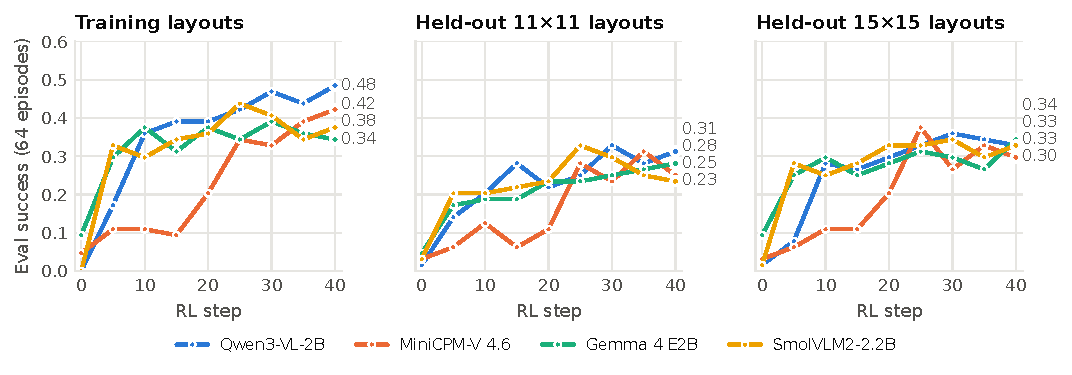
\includegraphics[width=\linewidth]{figures/maze_procgen.pdf}
\caption{Procedural mazes, 40 RL steps, sparse success reward. Eval success on training layouts and on held-out
layouts (same size, and larger 15$\times$15). Labels: final values.}
\label{fig:procgen}
\end{figure}
All four models improve on held-out layouts about as much as on training layouts, so they learn to navigate rather than
memorize layouts (Fig.~\ref{fig:procgen}). Learning rates matter by model: 5e-6 for Qwen3-VL-2B and SmolVLM2-2.2B,
1e-6 for Gemma 4 E2B and MiniCPM-V (5e-6 made MiniCPM-V near-deterministic within 3 steps).

\subsection{Single fixed mazes and the SmolVLM2-2.2B collapse}
\label{sec:fixed}
\begin{figure}[h]
\centering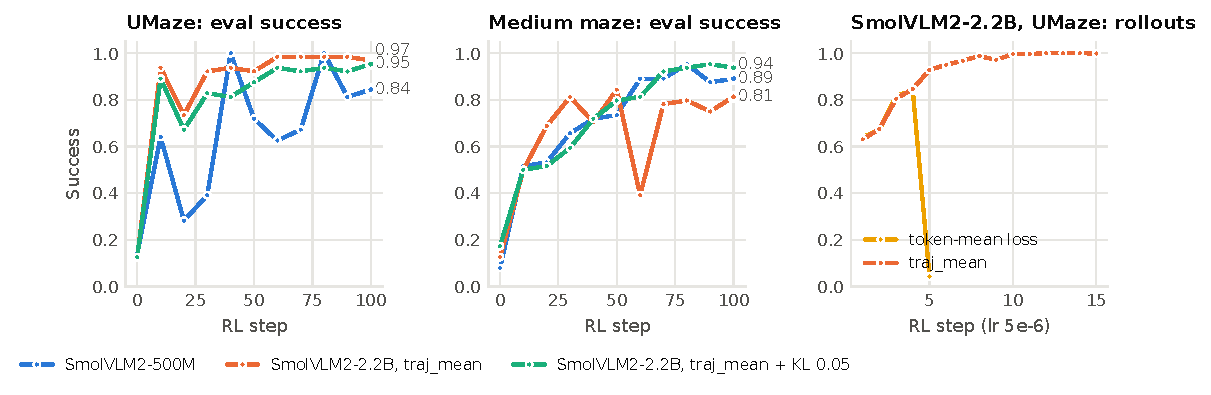
\includegraphics[width=\linewidth]{figures/maze_fixed.pdf}
\caption{Single fixed mazes, 100 steps. Left two: eval success. Right: SmolVLM2-2.2B training rollouts on UMaze with
the token-mean loss (collapses at step 5) and with \code{traj\_mean}.}
\label{fig:fixed}
\end{figure}
SmolVLM2-500M learns both fixed mazes (0.84 UMaze, 0.89 medium at step 100). SmolVLM2-2.2B with the default
token-mean loss collapses after a few updates (Fig.~\ref{fig:fixed}, right): success climbs to 0.84, the replies shrink from
98 to 22 characters, and the next update turns them into bare direction words (5 characters) that are not valid
actions, so success falls to 0.04 with 98\% invalid replies. The same happens on procedural mazes, so maze sampling is
not the cause; a lower learning rate, a warmup or a format penalty only delayed it.

\textbf{Why:} with a token-mean loss every token weighs the same. Failed episodes use all 20 turns while successful ones
are short, so failures carry most of the tokens and each update is net negative per token. That pushes probability away
from everything sampled, including the valid format. \textbf{Fix:} \code{traj\_mean} rescales advantages so every
trajectory weighs the same: UMaze 0.97, medium 0.81 (one dip at step 60); adding a small KL penalty to the reference
(0.05) also stabilizes medium (0.94).

\takeaway{Sparse success is enough for mazes, and the skill transfers to new layouts. If replies get shorter while
success rises, the loss is about to tip negative: weight trajectories, not tokens.}

%=====================================================================================================================
\section{Metaworld reach}

\subsection{RL alone works for Qwen3.5-4B}
\begin{figure}[h]
\centering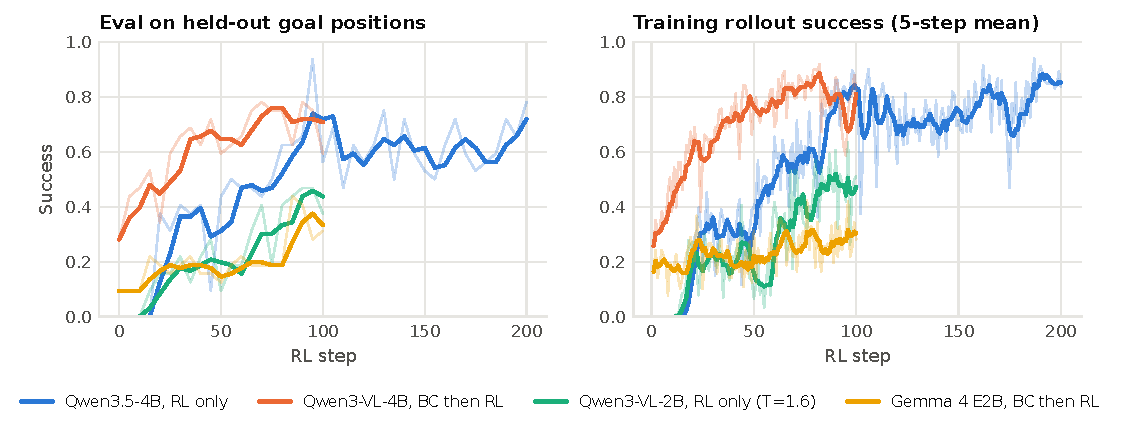
\includegraphics[width=\linewidth]{figures/reach_models.pdf}
\caption{ML1 reach. Left: eval on the 50 held-out goal positions (thin: each eval; thick: 3-eval mean). Right:
training-rollout success. BC runs start at their clone's score.}
\label{fig:reach}
\end{figure}
Qwen3.5-4B (LoRA on the MLPs, lr 1e-5, preference reward of Section~\ref{sec:pref}) starts at 0 and reaches 0.94 on
held-out goal positions at step 95; afterwards held-out plateaus at 0.5--0.78 while training positions reach 0.97
(0.78 / 0.88 at step 200). Zero-shot, every model scores 0.

\subsection{Exploration decides whether a model can start}
\begin{figure}[h]
\centering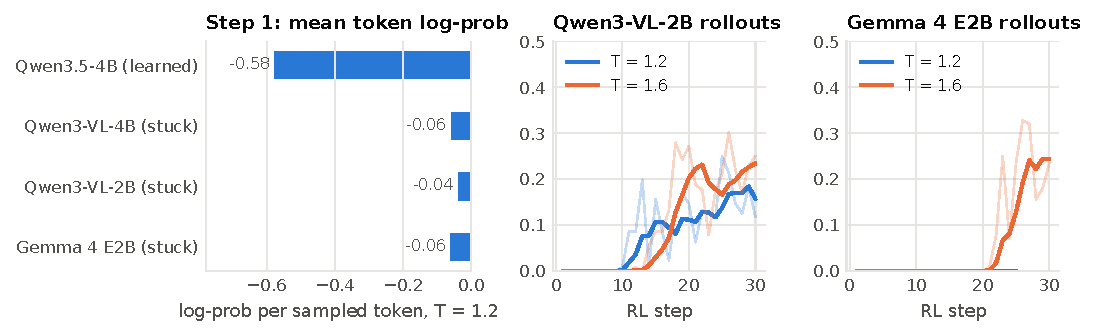
\includegraphics[width=\linewidth]{figures/reach_exploration.pdf}
\caption{Left: mean log-prob of the sampled tokens at the first RL step, all at temperature 1.2. Right: raising the
temperature to 1.6 lets two of the stuck models start.}
\label{fig:explore}
\end{figure}
The preference reward needs the 8 rollouts of a group to differ. Qwen3.5-4B samples diverse moves at temperature 1.2
(mean log-prob $-0.58$ per token at step 1); the other three are nearly deterministic ($-0.04$ to $-0.06$), so their
rollouts tie and the groups carry no signal (Fig.~\ref{fig:explore}). Raising the temperature to 1.6 got Qwen3-VL-2B
(RL only: 0.38 held-out at step 100, peak 0.47) and Gemma moving. Qwen3-VL-4B stayed stuck even at 2.0: it always
answered \code{dx = dy = 0}, never moving sideways.

\subsection{Behaviour cloning, then RL}
Metaworld ships a scripted expert per task. We drive it through the same text protocol, write its moves as the model's
replies, and fine-tune on the successful episodes (30 steps of 64 episodes), then run RL from the clone.
For Qwen3-VL-4B this turns 0 into the best reach model: 0.28 after cloning, 0.78 held-out (1.00 on training positions)
by step 70. Gemma 4 E2B goes from 0.09 to 0.31--0.44.

\takeaway{Check the step-1 log-prob before a long run: near zero means no exploration and no signal. Temperature
fixes moderate cases; cloning an expert fixes the rest, and RL then improves on the clone.}

%=====================================================================================================================
\section{Preference rewards from the ground truth}
\label{sec:pref}

\subsection{The recipe (\code{pref\_mw})}
Metaworld's success signal starts at 0\% for every model, so a sparse reward gives no signal. Instead each group is
turned into preferences from Metaworld's ground truth at the final state:
\begin{enumerate}
\item Score every rollout: $s = 10\cdot\text{success} + \log(0.001 + r_\text{final})$, where $r_\text{final}\in[0,10]$ is
  Metaworld's dense reward at the last step. An episode ended by an invalid reply gets $s=-20$.
\item Compare every pair: $P(i \succ j) = \sigma((s_i - s_j)/0.1)$, a tie if $|s_i - s_j| < 0.02$ (within 2\% on the
  log scale).
\item Each rollout's reward is its win rate against the other 7; GRPO z-scores these within the group.
\end{enumerate}
With temperature 0.1 on log rewards this is essentially a ranking by final progress, with success first.

\begin{table}[h]
\centering\small
\begin{tabular}{lrrrr}
\toprule
Rollout & $r_\text{final}$ & $s$ & Win rate & Advantage \\
\midrule
invalid reply & -- & $-20$ & 0 & $-1.34$ \\
no success & 0.03 & $-3.5$ & 1/3 & $-0.45$ \\
no success & 0.07 & $-2.6$ & 2/3 & $+0.45$ \\
success & 9.8 & 12.3 & 1 & $+1.34$ \\
\bottomrule
\end{tabular}
\caption{A worked example with 4 rollouts.}
\end{table}

\subsection{The grip-and-hold trap, and ranking by the object first}
\begin{figure}[h]
\centering
\begin{minipage}{0.5\linewidth}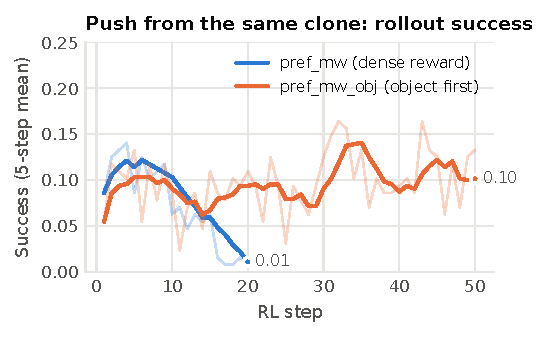
\includegraphics[width=\linewidth]{figures/push_reward.pdf}\end{minipage}\hfill
\begin{minipage}{0.47\linewidth}
\caption{Push, RL from the same cloned policy (controller gain 1.0). With the dense-reward ranking, success falls
from 0.11 to 0.01 in 15 steps; ranking by object progress first keeps it at $\sim$0.10.}
\label{fig:prefreward}
\end{minipage}
\end{figure}
On push, Metaworld's dense reward at the final state is about $1 + 2\cdot 2 + 5\cdot 0.1 \approx 5.5$ for
\emph{gripping the puck and holding it still}, but below 2 for pushing it partway and losing contact. The ranking therefore
rewards holding, and RL learned exactly that: descend, close the gripper on the puck, and stay for the rest of the
episode (Fig.~\ref{fig:prefreward}).

\code{pref\_mw\_obj} compares two rollouts rule by rule: (1) a valid ending beats an invalid one; (2) success wins; (3) the
rollout whose task object ended at least 1 cm closer to its goal wins (Metaworld's \code{obj\_to\_target}, for reach
the hand); (4) otherwise the dense-reward rule above.

\takeaway{A dense reward read at the final state is a fine ranking signal until it has a local optimum the policy can sit
in. Rank by the task's own progress measure (object to goal) before the shaped reward.}

%=====================================================================================================================
\section{Push: imitation, control, and generalization}

\subsection{RL alone finds nothing}
Every RL-only push run stayed at 0 (also from the trained reach adapter and at temperature 1.6): the policy repeats one
fixed move whatever the image shows, and never samples the sequence push needs (go behind the puck, drop, push).

\subsection{Cloning the expert, DAgger and DART}
\begin{figure}[h]
\centering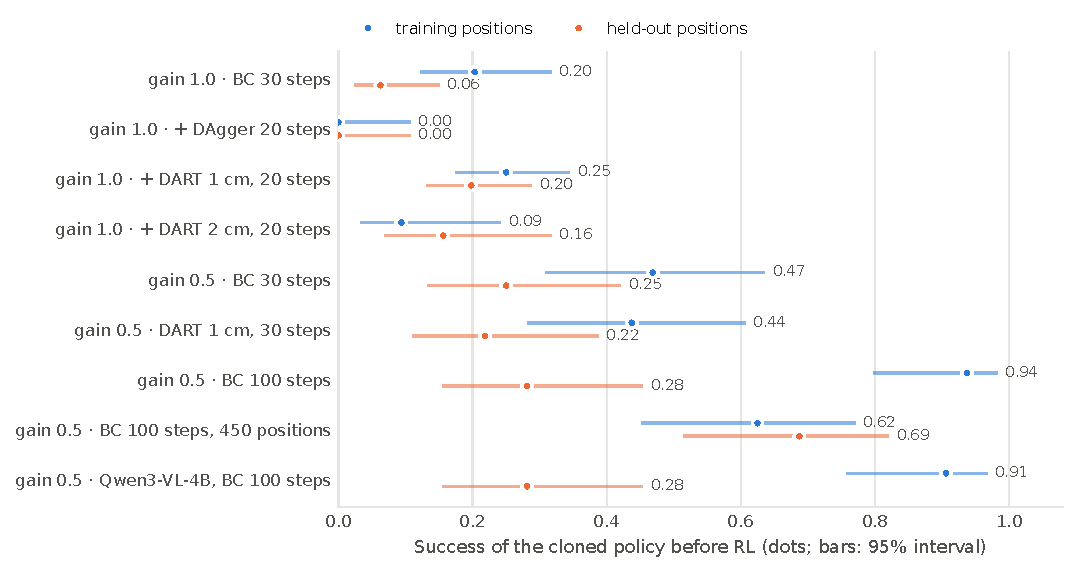
\includegraphics[width=\linewidth]{figures/push_clones.pdf}
\caption{Success of the cloned push policies before any RL (step-0 eval, 32 episodes per set; pooled where one recipe
has several evals). Bars: 95\% Wilson intervals.}
\label{fig:clones}
\end{figure}
\begin{table}[h]\centering\small\begin{tabular}{lrrl}
\toprule
Clone & Training pos. & Held-out pos. & Evals \\
\midrule
gain 1.0, BC 30 steps & 13/64 (0.20) & 4/64 (0.06) & two clones, same recipe \\
gain 1.0, + DAgger 20 steps & 0/32 (0.00) & 0/32 (0.00) &  \\
gain 1.0, + DART 1 cm, 20 steps & 24/96 (0.25) & 19/96 (0.20) & one clone, three evals \\
gain 1.0, + DART 2 cm, 20 steps & 3/32 (0.09) & 5/32 (0.16) &  \\
gain 0.5, BC 30 steps & 15/32 (0.47) & 8/32 (0.25) &  \\
gain 0.5, DART 1 cm, 30 steps & 14/32 (0.44) & 7/32 (0.22) &  \\
gain 0.5, BC 100 steps & 30/32 (0.94) & 9/32 (0.28) &  \\
gain 0.5, BC 100 steps, 450 positions & 20/32 (0.62) & 22/32 (0.69) & ablation \\
gain 0.5, Qwen3-VL-4B, BC 100 steps & 29/32 (0.91) & 9/32 (0.28) &  \\
\bottomrule
\end{tabular}
\caption{The same clones as counts (successes/episodes).}\end{table}

\textbf{Plain cloning} (30 steps) gave the first push successes: 0.20 on training positions, 0.06 held-out, against the
expert's 0.61 through the same protocol. The clone kept repeating the expert's ``drop onto the puck'' move after its hand
had already reached the table, a state the expert never visits.

\textbf{DAgger made it worse} (0.20 $\to$ 0.00). DAgger runs the clone and labels the states it reaches with the expert's
move. But Metaworld's experts are state machines with sharp thresholds on state the model cannot see: more than 2 cm from
the puck in $x/y$ means ``go back up 20 cm'', within 2 cm means ``drop and close''. In the clone's own states nearly
identical images got opposite labels; the fit to the labels fell to log-prob $-0.50$ (vs $-0.09$ on expert data).

\textbf{DART helped held-out positions a little}: the expert drives with 1 cm of noise on each move and its clean replies
are cloned, so the states stay near the expert's path but include small slips. Pooled over three evals, 19/96 held-out
successes vs 4/64 for the plain clone. With 2 cm of noise the expert's own success fell to 0.20 and the clone got worse.

\subsection{The controller gain}
\begin{figure}[h]
\centering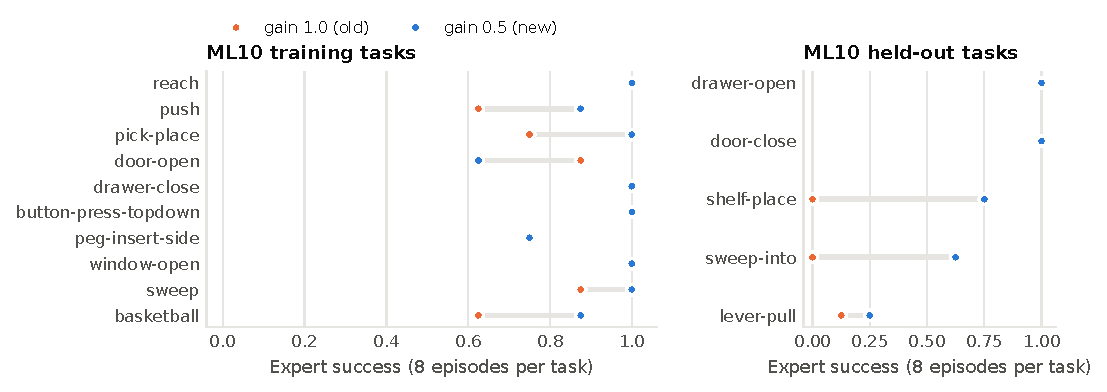
\includegraphics[width=\linewidth]{figures/expert_gain.pdf}
\caption{Scripted-expert success through our text protocol at the old and new controller gain (8 episodes per task;
where both dots coincide only one is visible). On ML1 push (30 episodes): 0.63 $\to$ 0.97.}
\label{fig:expert}
\end{figure}
The eval transcripts showed the clone doing the right thing (above the puck, drop, close, move 10 cm toward the goal)
while the hand rose 2--3 cm per turn during the drag, even though it was commanded down, until the puck slipped out.
The waypoint controller commanded full speed until 1 cm from each target (gain 1.0) and overshot. At gain 0.5 it slows
down from 2 cm out: the expert's push success goes from 0.63 to 0.97 and it needs 5.9 turns instead of 9.4. ML10's
experts improve too (training tasks 0.85 $\to$ 0.91, held-out tasks 0.42 $\to$ 0.72; only door-open drops,
Fig.~\ref{fig:expert}). The cloned push policy doubles (0.47 / 0.25 after 30 steps).

\subsection{More cloning: training positions solved, held-out positions not}
With 100 cloning steps both 4B models nearly solve push on its 50 training positions (Qwen3.5-4B 0.94, Qwen3-VL-4B 0.91),
but held-out stays at 0.28 for both, the same as after 30 steps. The fit to the expert data reaches log-prob $-0.003$:
the clone has memorized the 50 positions. ML1 push trains on only 50 puck/goal configurations.

An ablation outside the ML1 protocol clones on 450 positions (the training positions of benchmark seeds 0--9). This
needed care: \emph{seed 1's 50 training positions are exactly seed 0's 50 held-out positions}, so any training position within
1 cm of a held-out one is dropped. The remaining positions sit closer to the held-out ones (median nearest distance 2.2 cm
instead of 3.8 cm), which has to be kept in mind when reading the result.

\textbf{Result: the gap closes.} The 450-position clone scores 0.62 on training positions and \textbf{0.69 on held-out
positions} (from 0.28), with a fit of $-0.155$ instead of $-0.003$: it can no longer memorize, so it learns the task.
Denser coverage alone would not explain a jump from a 0.66 gap to none.

\subsection{RL from the clones}
\begin{figure}[h]
\centering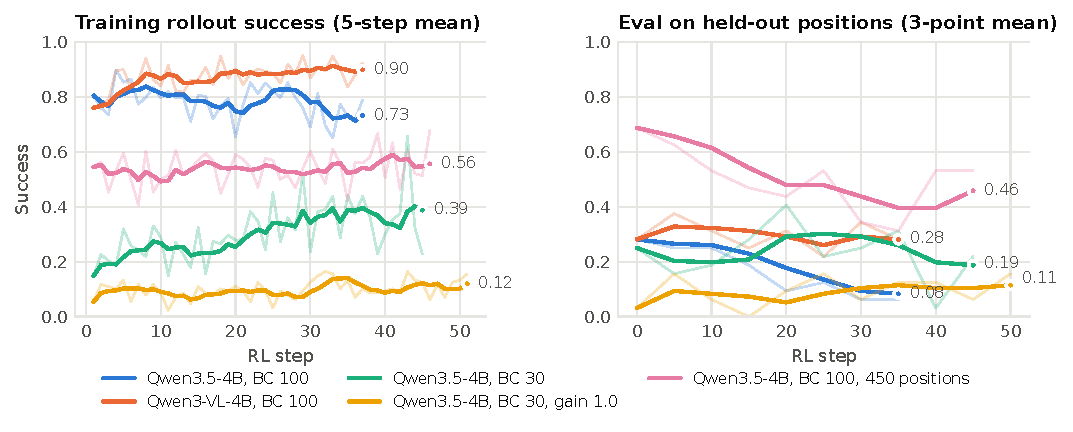
\includegraphics[width=\linewidth]{figures/push_rl.pdf}
\caption{Push, RL from the cloned policies (\code{pref\_mw\_obj}, temperature 1.0 except the gain-1.0 run at 1.2).}
\label{fig:pushrl}
\end{figure}
At gain 0.5, RL improves the 30-step clone: training rollouts rise from 0.22 (steps 1--5) to 0.36 (steps 36--45); at
gain 1.0 they never left $\sim$0.10. From the memorized 100-step clones, rollouts stay at 0.8--0.9 and held-out does not
improve: Qwen3.5-4B drifts from $\sim$0.26 to $\sim$0.08 over 35 steps, Qwen3-VL-4B stays at 0.2--0.35
(Fig.~\ref{fig:pushrl}). RL on the 50 training positions sharpens the memorized behaviour rather than generalizing it.

\textbf{RL from the good 450-position clone does not help either, so far.} Training rollouts stay flat (0.54 over steps
1--5, 0.53 over steps 31--40) while the sampled replies get more deterministic (mean log-prob of sampled tokens $-0.19
\to -0.14$), and held-out positions fall steadily: 0.69, 0.62, 0.53, 0.47, 0.44, 0.53, 0.34, 0.31 at steps 0--35. RL
sharpens the policy on what it samples instead of improving it.

\textbf{Lower learning rate, or positive-only advantages?}
\begin{figure}[h]
\centering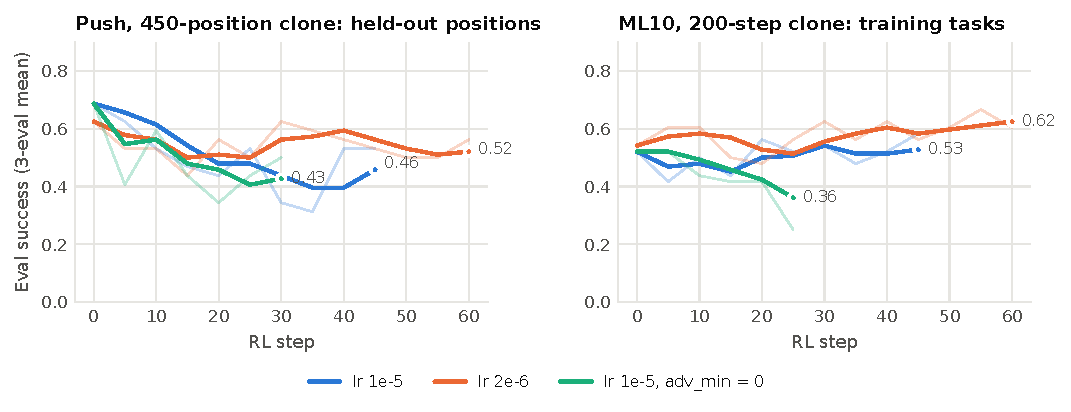
\includegraphics[width=\linewidth]{figures/rl_fixes.pdf}
\caption{RL from the 450-position push clone and the 200-step ML10 clone at three settings (thin: each eval; thick:
3-eval mean).}
\label{fig:rlfixes}
\end{figure}
From the same two clones, RL at a 5$\times$ lower learning rate (2e-6), and RL reinforcing only above-average rollouts
(\code{adv\_min=0}, so it never pushes probability away from a sampled move), compared with lr 1e-5
(Fig.~\ref{fig:rlfixes}). Pooled over the evals at steps 5--15:

\begin{center}\small
\begin{tabular}{lrr}
\toprule
RL setting & Push, held-out positions & ML10, training tasks \\
\midrule
clone (step 0) & 0.62--0.69 & 0.52--0.54 \\
lr 1e-5 & 0.54 & 0.45 \\
lr 2e-6 & 0.50 & 0.57 \\
lr 1e-5, \code{adv\_min=0} & 0.48 & 0.46 (0.34 at steps 20--30) \\
\bottomrule
\end{tabular}
\end{center}

Positive-only advantages are worse on ML10: in a group where every rollout fails, the above-average failures are still
reinforced (rollouts 0.44 $\to$ 0.30). The lower learning rate holds up better the longer it runs: pooled over steps
20--30, held-out push is 0.56 at lr 2e-6 against 0.44 at lr 1e-5 (clone 0.62), and ML10's training tasks stay at 0.55
(steps 5--25) against 0.45--0.54. Over 50--60 steps at lr 2e-6, RL slowly improves what it trains on: ML10 rollouts rise
from 0.49 (steps 1--10) to 0.64 (steps 41--50), push rollouts from 0.53 to 0.66 (steps 51--60). Greedy evals move less (ML10
training tasks 0.54 $\to$ 0.56--0.59, push training positions 0.62 $\to$ 0.73), and held-out push stays slightly below the
clone (0.51--0.57 against 0.62). At lr 2e-6 RL refines a good clone on its training distribution; it does not add
generalization.

\textbf{Temperature for RL from a clone.} Unlike reach from scratch, a clone already varies its moves, and sampling
noise in the digits spoils precise pushes. From the same DART clone, mean rollout success over the first 9 steps was
0.106 at temperature 0.8 and 1.0 and 0.060 at 1.2.

\takeaway{Before blaming the model, run the scripted expert through your own action interface: our controller capped the
expert at 0.63. Cloning then gets training positions to $>$0.9, but with 50 configurations the model memorizes them;
cloning on 450 positions closes the held-out gap (0.28 $\to$ 0.69). Generalization comes from varied data, not from
more RL on the same positions.}

%=====================================================================================================================
\section{ML10: a wider task distribution}
\label{sec:ml10}
\begin{figure}[h]
\centering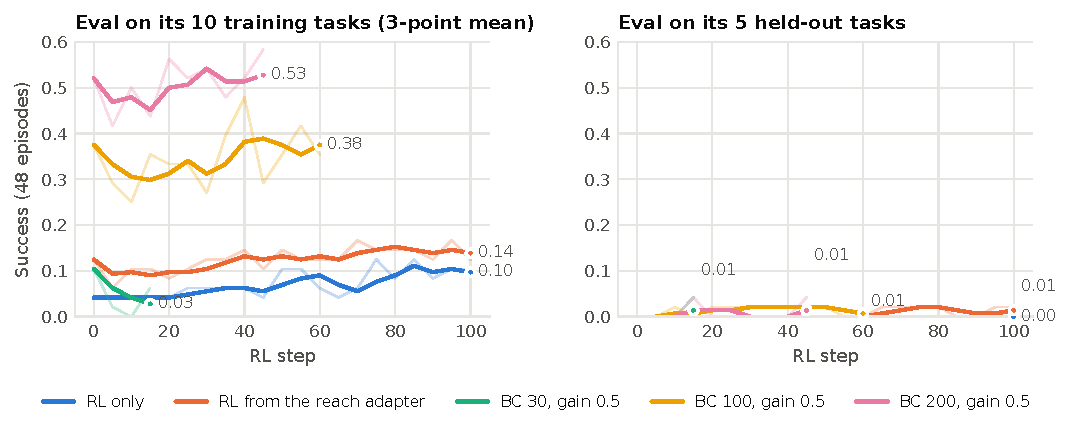
\includegraphics[width=\linewidth]{figures/ml10.pdf}
\caption{ML10 with Qwen3.5-4B: eval on its 10 training tasks and its 5 held-out tasks (48 episodes each).}
\label{fig:ml10}
\end{figure}
RL alone reaches 0.10--0.12 on the training tasks; starting from the trained reach adapter, 0.12--0.17, with the first
held-out-task successes (0.02). Cloning needs many more steps than on one task:

\begin{center}\small
\begin{tabular}{lrr}
\toprule
ML10 clone (Qwen3.5-4B, gain 0.5) & Training tasks & Fit (log-prob) \\
\midrule
30 BC steps & 0.10 & $-0.35$ \\
100 BC steps & 0.38 & $-0.18$ \\
200 BC steps & 0.52 & $-0.04$ \\
recipe: 200 BC steps, 500 variations per task & 0.54 & $-0.24$ \\
recipe: 400 BC steps, 500 variations per task & 0.69 & $-0.19$ \\
\bottomrule
\end{tabular}
\end{center}

RL from the 100-step clone moved its eval within noise (0.27--0.48 over 60 steps). From the 200-step clone RL keeps it
level: training-task eval 0.42--0.56 against the clone's 0.52, rollouts 0.47--0.50 per 10 steps, and the sampled-token
log-prob unchanged ($-0.155$). At this scale RL adds nothing measurable on top of cloning; the clone's quality, set by how
much expert data it saw, is what moves ML10. The 5 held-out tasks stay near 0 in every run: the instructions and objects are new, and 10 training tasks
are too few to transfer.

\takeaway{Multi-task cloning scales with the number of tasks: budget proportionally more expert data. Held-out
\emph{tasks} (as opposed to held-out positions) did not work at all at this scale.}

%=====================================================================================================================
\section{The recipe for ML10 and ML45 (running)}
Everything that worked is generic: nothing in it is written per task.
\begin{enumerate}
\item Controller gain 0.5 (one environment setting).
\item Behaviour cloning on Metaworld's own scripted experts, driven through the text protocol, with the number of
  steps scaled to the number of tasks.
\item Training variations from 10 benchmark seeds (\code{env\_kwargs.train\_seeds=10}, 500 per task). ML10/ML45's
  held-out tasks are other task classes, so extra variations of the training tasks cannot leak into them.
\item RL with \code{pref\_mw\_obj} at temperature 1.0 (it uses only quantities every Metaworld task reports). This
  step is optional so far: from good clones RL has kept ML10 level and lowered held-out push (Fig.~\ref{fig:rlfixes}). The recipe runs use lr 1e-5; their saved clones also get RL at lr 2e-6 for comparison.
\end{enumerate}
It is packaged as one sweep (\code{configs/sweeps/metaworld\_recipe.yaml}) for ML10 (200 cloning steps) and ML45 (400).

\textbf{ML10 clone from the recipe:} 0.54 on the training tasks and 0.02 on the held-out tasks, with a fit of $-0.24$.
The 200-step clone on the benchmark's own 50 variations per task scored 0.52 at a fit of $-0.04$, on the same eval
variations it had trained on; the recipe's clone matches it without memorizing them. RL from it, 20 steps in: training
tasks 0.56 (lr 1e-5) and 0.62 (lr 2e-6), pooled over steps 5--20; the same clone's step-0 evals were 0.54 and 0.60, so the
two are not yet distinguishable. Later RL improves the clone at both learning rates: pooled over steps 30--50, training
tasks reach 0.68 (lr 1e-5) and 0.66 (lr 2e-6) against the clone's 0.57; held-out tasks stay at 0.00--0.06. Unlike push,
lr 1e-5 does not erode anything here.

\begin{figure}[h]
\centering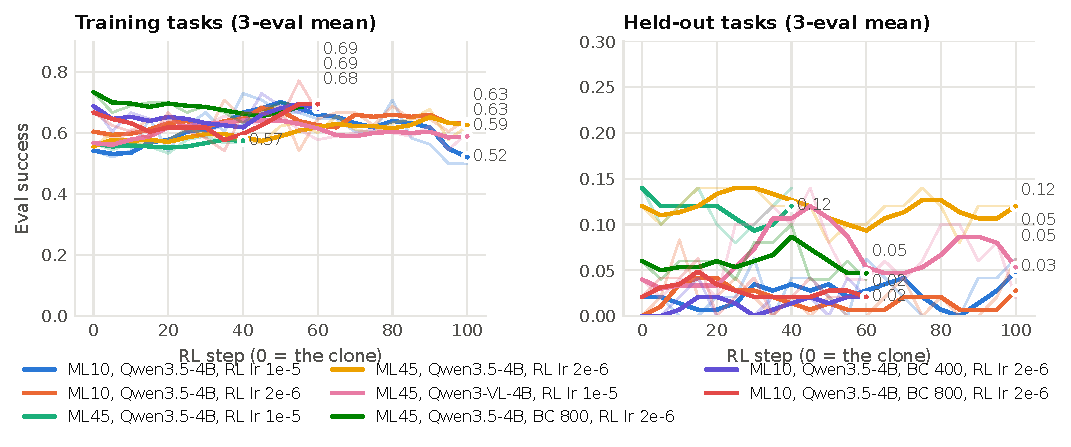
\includegraphics[width=\linewidth]{figures/recipe.pdf}
\caption{The generic recipe on ML10 and ML45. Step 0 is the cloned policy; RL follows (thin: each eval; thick: 3-eval
mean). Training tasks: 48 (ML10) / 90 (ML45) episodes per eval; held-out tasks: 48 / 50.}
\label{fig:recipe}
\end{figure}

\textbf{ML45 clone from the recipe} (Qwen3.5-4B, 400 cloning steps): 0.57 on the 45 training tasks (the experts' ceiling
through our protocol is 0.82) and \textbf{0.14 on the 5 held-out tasks}, without ever seeing them (7 of 50 episodes; 95\%
interval 0.07--0.26). ML10's clones, trained on 10 tasks, scored 0.00--0.02 on theirs. This is the first sign that
cloning many tasks transfers to new ones; it holds across six evals of the same clone (0.10--0.14). The same recipe with
Qwen3-VL-4B gives 0.57 on the training tasks but only 0.04 on the held-out ones: Qwen3.5-4B transfers better.

RL barely moves ML45 (Fig.~\ref{fig:recipe}): at lr 2e-6 the Qwen3.5-4B clone goes from 0.57 to 0.63 on the training
tasks (pooled over steps 65--85) and stays at 0.08--0.14 on the held-out ones. Over 100 steps on ML10, lr 1e-5 peaked at
0.71 (step 80) and then fell to 0.54 (steps 85--100), while lr 2e-6 held 0.64: lr 2e-6 is the safe setting.

\textbf{More cloning beats RL on the training tasks.}

\begin{center}\small
\begin{tabular}{lrrr}
\toprule
Recipe clone (Qwen3.5-4B) & Training tasks & Held-out tasks & Fit \\
\midrule
ML10, 200 BC steps & 0.54 & 0.02 & $-0.24$ \\
ML10, 400 BC steps & \textbf{0.69} & 0.00 & $-0.19$ \\
ML10, 800 BC steps & 0.67 & 0.02 & $-0.11$ \\
ML45, 400 BC steps & 0.57 & 0.12 (pooled, 6 evals) & $-0.19$ \\
ML45, 800 BC steps & \textbf{0.73} & 0.056 (14/250, 5 evals) & $-0.17$ \\
\bottomrule
\end{tabular}
\end{center}

Doubling the cloning lifts the training tasks by 0.15 on both benchmarks, as much as or more than RL ever did, and ML45's
800-step clone (0.73) comes close to its experts' 0.82. ML10 saturates between 400 and 800 steps (0.69, 0.67) although
the fit keeps improving ($-0.19 \to -0.11$) and its experts reach 0.91: something other than the amount of expert data
limits it now. Per-task evals of the saved clones are running to show which tasks fail. \textbf{Held-out tasks go the other way}: pooled over five evals,
the 800-step ML45 clone transfers 0.056 (14/250) against the 400-step clone's 0.12 (36/300; $p\approx0.01$). Cloning
longer fits the training tasks at the cost of transfer, so the checkpoint that transfers best is not the one that scores
best on the training tasks. RL from either clone leaves both numbers where cloning put them (ML10 400-step clone: 0.62--0.73
over 60 RL steps, against 0.69).
ML45's scripted experts, at gain 0.5 through the same protocol, succeed 0.82 on its 45 training tasks (handle-pull-side,
lever-pull and stick-push at 0) and 0.97 on its 5 held-out tasks: the ceiling for this recipe.

\subsection{Task by task}
\begin{figure}[p]
\centering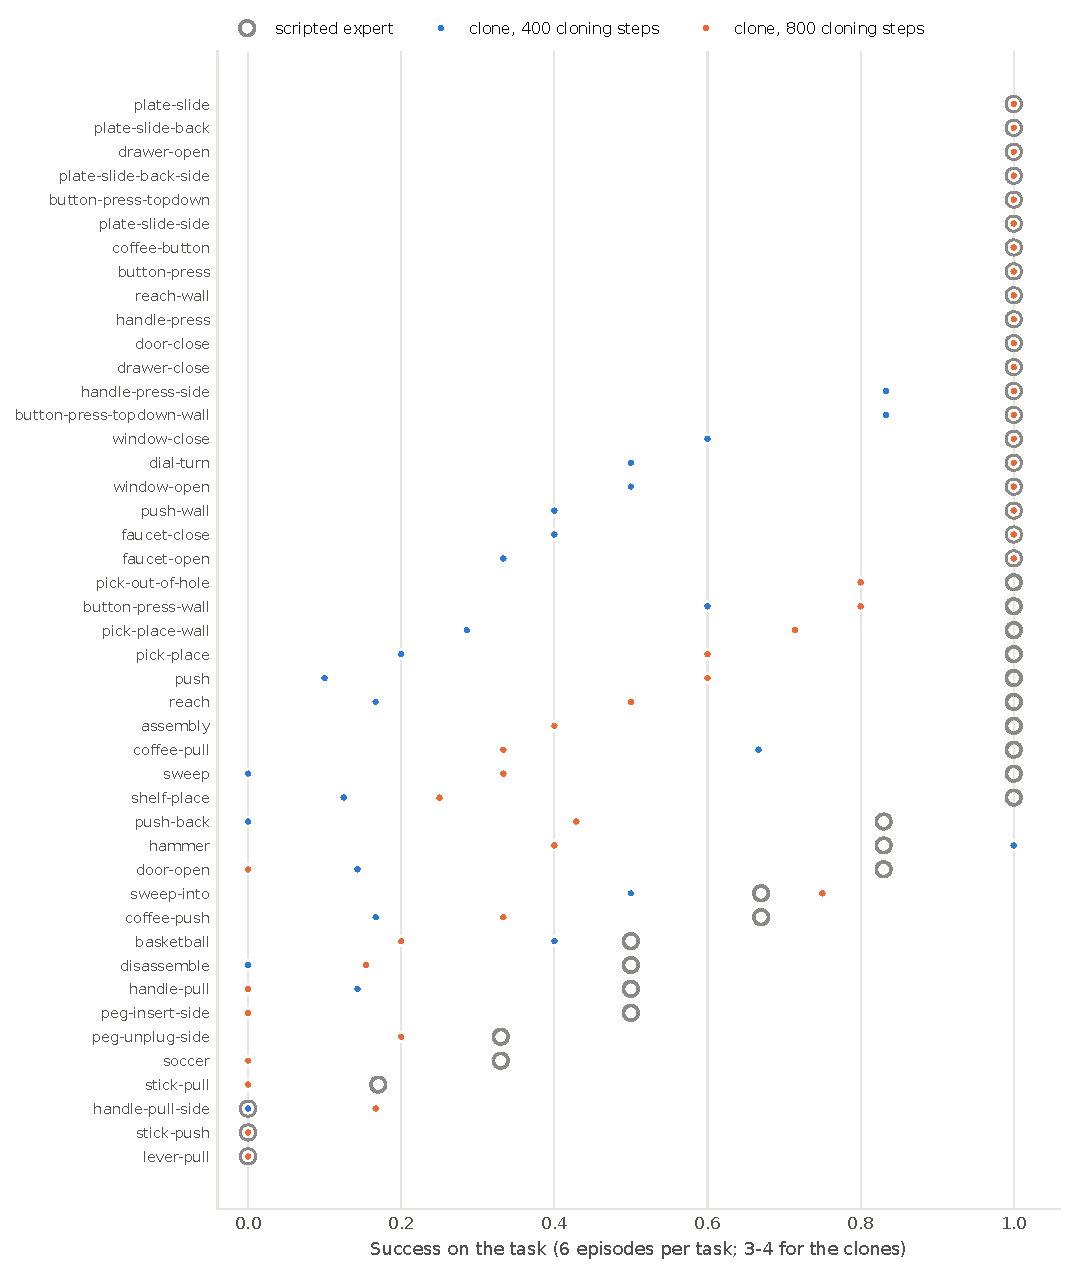
\includegraphics[width=\linewidth]{figures/pertask_ml45.pdf}
\caption{ML45 training tasks: success of the scripted expert (ring; our protocol, gain 0.5) and of the 400- and 800-step
clones (eval only, 270 episodes in all). Where both clones are at 1.0 only the later dot is visible.}
\label{fig:pertask45}
\end{figure}
\begin{figure}[h]
\centering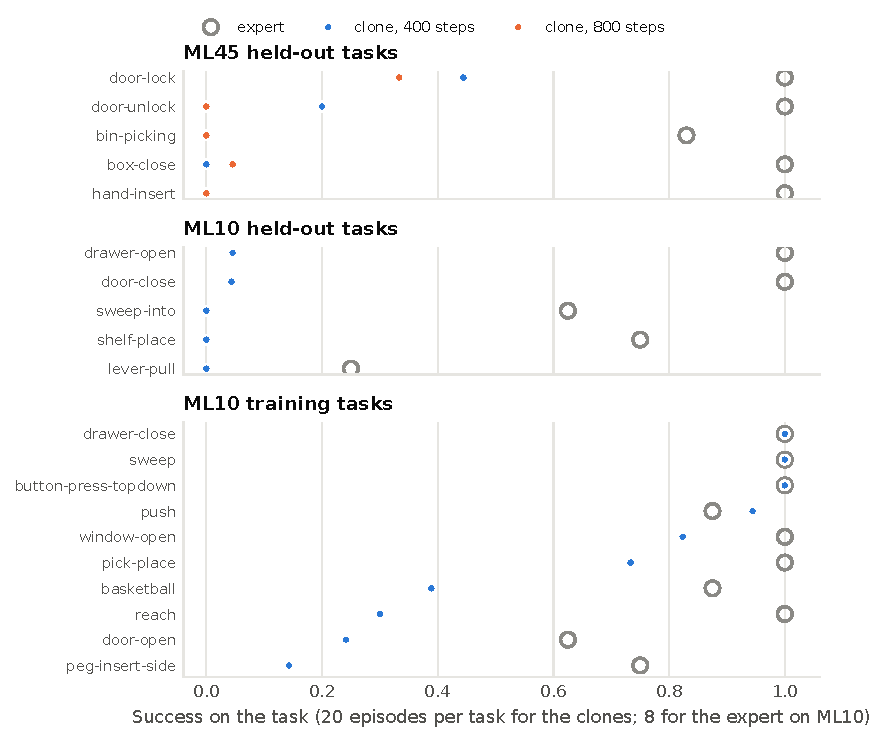
\includegraphics[width=0.8\linewidth]{figures/pertask_heldout.pdf}
\caption{Held-out tasks of ML45 and ML10, and ML10's training tasks (20 episodes per task for the clones).}
\label{fig:pertaskho}
\end{figure}
Per-task evals of the saved clones (Figs.~\ref{fig:pertask45}, \ref{fig:pertaskho}) show where the scores come from:
\begin{itemize}
\item \textbf{Some training-task zeros are the expert's.} The scripted expert itself fails handle-pull-side, lever-pull and
  stick-push through our protocol (and stick-pull 0.17); no amount of cloning fixes these. The others are the model's:
  sweep, push-back and disassemble are 0 at 400 cloning steps with experts at 0.5--1.0.
\item \textbf{Longer cloning trades tasks for tasks.} From 400 to 800 steps, push goes 0.10 $\to$ 0.60, pick-place 0.20
  $\to$ 0.60, sweep 0 $\to$ 0.33 and 12 tasks reach 1.0, but door-open (0.14 $\to$ 0), handle-pull, coffee-pull, basketball
  and hammer get worse.
\item \textbf{Held-out transfer comes from look-alike tasks.} On ML45 only door-lock (0.44 / 0.33) and door-unlock (0.20 /
  0.00) transfer: their objects and motions resemble training tasks (doors, dials, handles). Bin-picking, box-close and
  hand-insert stay at 0.
\item \textbf{Unseen motions fail.} ML10 trains on drawer-close and door-open; its held-out tasks drawer-open and
  door-close are their opposites, and the clone almost never solves them (0.05, 0.04). The policy does read the
  instruction (Section~\ref{sec:scale}: with swapped instructions its training-task success halves), so these fail because
  no training task demonstrated pulling a drawer or pushing a door shut. Even ML10's reach is only 0.30 although its expert
  is perfect.
\end{itemize}

\section{Reasoning for generalization (in progress)}
\label{sec:reasoning}
Held-out tasks need the policy to work out what a new instruction asks for, which is what reasoning should help with.
The obstacle: everything that works so far is cloned from Metaworld's scripted experts, whose data has no reasoning
(image in, move out), so cloning trains direct answers.

\textbf{Native thinking does not produce actions.} Qwen3.5-4B with its thinking mode on (4096 tokens per reply, eval only
on ML45): 0.00 on the training and the held-out tasks; 87\% of replies are invalid and episodes end after 1.3 turns. The
reasoning is sensible (it finds the bins, the cube and the gripper and plans a move) but it loops (``Wait, I think I'm
just stuck in a loop'') and is cut off before it closes the thinking block. The 400-step ML45 clone with thinking on does
no better (0.02 / 0.00, against 0.57 / 0.12 without). Without thinking the base model gives valid moves every turn but no
successes. Native thinking would need a hard token budget.

\textbf{Bounded reasoning in the reply} (\code{prompt\_style=compact\_rel\_reason}): one or two sentences about where the
gripper, the object and the goal are, then the JSON move; the last \code{\{...\}} is parsed. Every reply is valid. The base
model describes scenes correctly (``the gripper is above the red bin, which contains a green cube; the goal is the blue
bin'') but its moves are timid or wrong: 0.01 on the training tasks, 0 held-out. The 400-step clone under this prompt
writes short, relevant reasons and expert-like moves, but loses most of its skill (0.12 / 0.06, against 0.57 / 0.12
with its own prompt): it was trained on answer-only replies.

\textbf{Cloning with reasons} (\code{bc\_rationale}). So the two have to be trained together. Each expert reply is
prefixed with a reason written by the base model when shown the observation and the expert's move (STaR-style
rationalization); training uses the normal prompt, so the clone learns ``reason, then move''. The test is whether the
instruction then steers the motion: ML10's drawer-open and door-close (the opposites of its training tasks, 0.05 and
0.04 for the answer-only clone) and ML45's held-out tasks.

\textbf{First attempt: worse, because of the reasons.} The ML45 clone with reasons (400 cloning steps) scores 0.34 on the
training tasks and 0.04 on the held-out ones, against 0.57 / 0.12 for the answer-only clone. Its replies show why: the base
model, asked why the expert's move was right, often answered that it was \emph{wrong} (``The proposed move is incorrect
because it attempts to move the gripper far away\ldots''; the experts' moves exceed the prompt's 10 cm and are shortened
by the environment), and the other reasons were long and generic (``adjust the gripper slightly to align it''). The clone
learned to say a move is incorrect and then make one.

\textbf{On ML10 the same flawed reasons still help the held-out tasks.} With reasons, the ML10 clone (400 cloning steps,
per-task eval) scores 0.51 on the training tasks (answer-only 0.61) but \textbf{0.07 on the held-out tasks} (answer-only
0.02; 7/100 vs 2/100, $p \approx 0.09$). Door-close, the opposite of the training task door-open, rises from 0.04 to 0.17;
lever-pull and sweep-into from 0 to 0.06. On the training tasks reasoning helps where reading the scene and the instruction
matters (door-open 0.24 $\to$ 0.55, reach 0.30 $\to$ 0.45) and hurts precise manipulation (pick-place 0.73 $\to$ 0.13, push
0.94 $\to$ 0.33). A first sign that reasoning helps with new instructions, which the cleaner second attempt did not confirm.

\textbf{Reasoning learned by RL instead of copied.} RL alone from the base model, with the short-reasoning prompt and
no cloning (lr 1e-5, temperature 1.0), starts at 0.01 on the training tasks. By step 30 it solves drawer-close (0.93)
and transfers to the held-out door-close at 0.52 (Fig.~\ref{fig:reasoningml10}); held-out tasks overall 0.12, the best on
ML10 so far, against 0.02 for every answer-only clone.
Nobody wrote its reasons; RL found that stating what the instruction
means for the motion pays: ``The door is open and needs to be pushed shut. The hand should move to the right to push the
door closed.'' $\to$ \code{dx +5} $\to$ success. It is still poor at the other tasks after 30 steps (training tasks
0.07): the motor skill that cloning gives has to be learned from scratch. RL on the first reasoning clone stayed flat
(held-out 0.06 at step 20).

\textbf{It did not hold.} At step 40 held-out door-close is 0.04 and held-out tasks overall 0.01, while the training tasks
keep improving (0.10: drawer-close 1.00, reach 0.20, window-open 0.18). The reasoning is unchanged in kind (``The door is
open and needs to be pushed shut. The gripper should move to the right''); the moves are not: the clean \code{dx +5} pushes
of step 30 now carry forward and downward components (\code{dy +2}, \code{dz -1}) learned on the training tasks, and the
door is sometimes judged angled the other way. RL on the training tasks reshapes the motion they share with the held-out
task, and the transfer it found along the way was not kept. By step 60 the training tasks have stalled at 0.10 (one task
solved, two at 0.2) and held-out tasks are at 0. Keeping such transfer would need held-out-aware checkpoint selection, a
smaller learning rate or a broader task mix, none of which has been tried yet. On ML45, RL from the base model gets no
signal at all (rollouts 0.00--0.01 over 23 steps, stopped): with 45 tasks a policy that solves none of them rarely
produces a better rollout to reinforce, so on the large benchmark reasoning has to start from a clone.

\begin{figure}[h]
\centering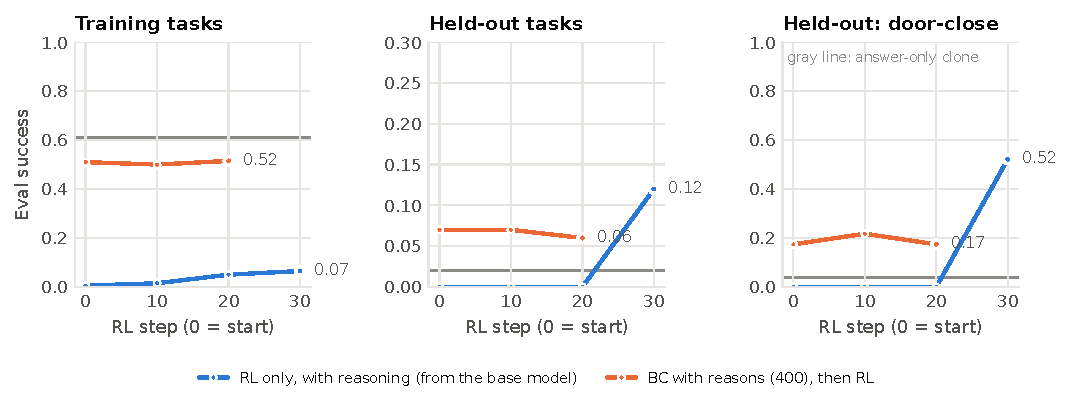
\includegraphics[width=\linewidth]{figures/reasoning_ml10.pdf}
\caption{ML10 with reasoning in every reply: RL only from the base model, and RL after cloning with reasons (gray line:
the answer-only 400-step clone). Training tasks 200, held-out tasks 100 episodes per eval.}
\label{fig:reasoningml10}
\end{figure}

\textbf{Second attempt at cloning with reasons} (one sentence of at most 25 words about where the gripper is relative to
the object and the goal, never judging the move): on ML45 it restores the skill (training tasks 0.47 against 0.49 for the
answer-only clone on the same per-task eval, and 0.34 for the first attempt; no invalid replies) but not transfer
(held-out tasks 0.05 against 0.12: door-lock 0.22 vs 0.44, door-unlock 0.05 vs 0.20). On ML45, cloned reasoning does not help
held-out tasks. On ML10 the second attempt matches the answer-only clone on the training tasks (0.62 vs 0.61) and on the
held-out ones (0.03 vs 0.02; door-close 0.09 vs 0.04): the first attempt's held-out gain (0.07) did not survive cleaner
reasons. Cloned reasoning has not reliably improved transfer on either benchmark.

\textbf{GRPO vs REINFORCE++.} Our loss is REINFORCE already; what makes it GRPO is the advantage: each group's rewards
are divided by that group's standard deviation, so a group of near-equal rollouts gets full-size advantages.
REINFORCE++-baseline (\code{adv\_mode=reinforce\_pp}) subtracts the group mean and divides by the standard deviation of the
whole batch instead, so near-tied groups barely move the policy. Run as twins with identical settings from the 400-step
clones (lr 2e-6, Fig.~\ref{fig:advmode}), the two are indistinguishable: pooled over steps 10--40, ML10's training tasks
0.64 (REINFORCE++) vs 0.63 (GRPO) and held-out 0.01 vs 0.03; ML45's 0.53 vs 0.52 and 0.13 vs 0.12. Neither erodes the clone
at this learning rate, so the earlier erosion came from the learning rate, not the normalization. For RL-only reasoning on
ML10 REINFORCE++ is slightly slower (training tasks 0.03 at step 30, GRPO 0.07). REINFORCE++'s token-level KL to the
starting model was not included (with LoRA our KL reference is the base model, not the clone).

\begin{figure}[h]
\centering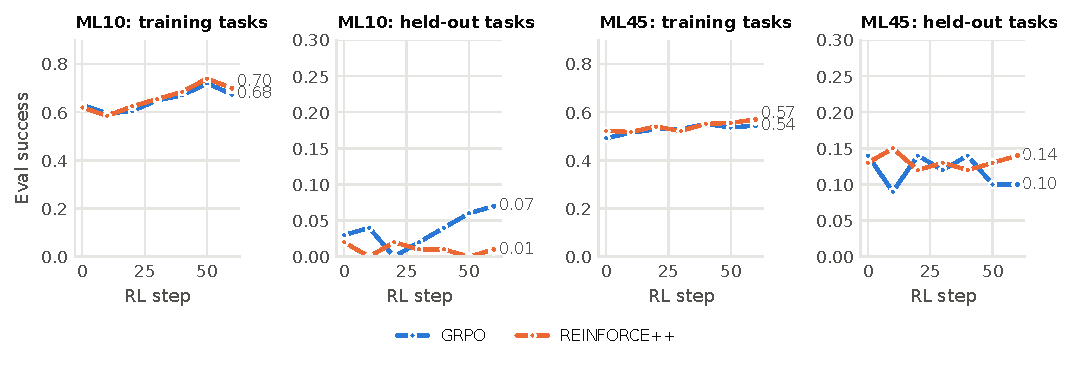
\includegraphics[width=\linewidth]{figures/advmode.pdf}
\caption{GRPO and REINFORCE++-baseline advantages, RL from the same 400-step clones with identical settings.}
\label{fig:advmode}
\end{figure}

\section{Is cloning necessary? RL alone on ML10}
\label{sec:rlonly}
\begin{figure}[h]
\centering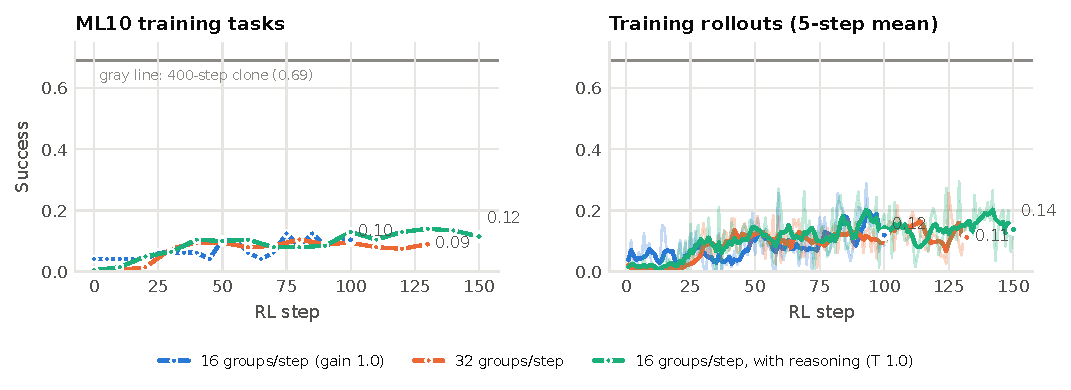
\includegraphics[width=\linewidth]{figures/rlonly_ml10.pdf}
\caption{RL from the base model (no cloning) on ML10: 16 groups per step (the first ML10 run, controller gain 1.0),
32 groups per step (twice the signal per task, temperature 1.2) and RL-only reasoning. Eval: 48 or 200 episodes.}
\label{fig:rlonly}
\end{figure}
Without cloning, RL has learned one or two ML10 tasks: drawer-close (1.00 by step 40) and a little reach (0.10--0.25).
Doubling the groups per step to 32 (about three per task) has not changed that through step 170 of 300 (training tasks
0.08--0.10 from step 40 on, the same as with 16 groups; held-out 0--0.01), so the plateau is not for lack of samples. The base model scores
$\approx$0 everywhere, and multi-phase motions (grasp, then place) are never sampled. This run continues to 300 steps.
On ML45, RL from the base model got no signal at all. So far cloning, or another source of motor skills, is necessary.

\section{Would a larger model generalize?}
\label{sec:scale}
Qwen3.5-4B and Qwen3-VL-4B are the same size and reach the same 0.57 on ML45's training tasks with the same recipe, yet
transfer 0.12 vs 0.04: at this scale pretraining matters more than parameter count. Two tests:
\begin{itemize}
\item \textbf{Scale: no gain so far.} Qwen3.5-9B (same family and architecture, 2.3$\times$ the parameters) with the same
  recipe (\code{policy=qwen35\_9b\_lora\_mlp}, 400 cloning steps). On ML45, with the same per-task eval as the 4B clone:
  0.51 on the training tasks (4B: 0.49) and 0.08 on the held-out ones (4B: 0.12; door-lock 0.22 vs 0.44, door-unlock 0.10 vs
  0.20, box-close 0.09 vs 0). Twice the parameters give the same fit and the same narrow transfer, as expected if held-out
  tasks fail for lack of demonstrated motions. On ML10 the 9B fits the training tasks a little better (0.67 vs 0.61:
  door-open 0.55 vs 0.24, reach 0.60 vs 0.30) and transfers exactly as little (held-out 0.02; drawer-open 0.05, door-close
  0.04, the same as the 4B).
\item \textbf{Does the clone read the instruction? Yes.} The 4B clones evaluated with every task given another task's
  instruction (\code{env\_kwargs.swap\_instructions=true}): ML45's training tasks fall from 0.49 to 0.11 and ML10's from 0.61
  to 0.28 (sweep 1.00 $\to$ 0, window-open 0.82 $\to$ 0; drawer-close, told to pull the drawer open, 1.00 $\to$ 0.57, as it
  partly obeys). So the policy follows the instruction. When drawer-open is the actual task it still fails (0.05) because no
  training task ever showed it how to pull a drawer: held-out failures are missing \emph{motions}, not ignored language.
  This corrects the earlier reading of the per-task results (Fig.~\ref{fig:pertaskho}).
\end{itemize}

\section{Why doesn't RL generalize here the way it does for frontier LLMs?}
Frontier RL on LLMs improves held-out problems. Four differences explain why ours does not, and model size is not among
them (Section~\ref{sec:scale}):
\begin{enumerate}
\item \textbf{Breadth.} Frontier RL trains on millions of problems, so a held-out problem shares structure with many
  training ones. We have 10 or 45 tasks, and transfer is exactly that narrow: only to look-alikes (door-lock from door and dial
  tasks), more with 45 tasks than with 10.
\item \textbf{What RL starts from.} Frontier RL mostly elicits and sharpens what the base model can already do, which
  needs some success to start from. Our base model scores $\approx$0 on every task (no prior for this arm and this action
  interface), so every motor skill comes from our training tasks; on ML45, RL from the base model got no signal at all.
\item \textbf{Missing motions, not missing understanding.} The clones follow the instruction (the swap test) but fail
  held-out tasks whose motion no training task demonstrated.
\item \textbf{No memory within an episode.} A frontier model tries, sees the result and revises in context. A
  one-frame policy cannot even remember what it was told about the goal or what it has done. Section~\ref{sec:goalhist}
  gives it the text history; that alone produced our largest held-out gain so far.
\end{enumerate}

\section{Goal once in text, with the text history}
\label{sec:goalhist}
Metaworld's ML benchmarks hide the goal from the state vector; our VLM sees it only as the goal marker in the image.
Here the first turn also states the goal relative to the hand, in the move's own units (\code{Goal: dx=+71.0, dy=+14.1,
dz=-4.6 from the hand}, \code{prompt\_style=compact\_rel\_goal}), and every earlier turn's text stays in context
(\code{max\_frames=null}, \code{max\_images=1}: only the latest image). The marker is unchanged. Everything else is the
recipe: 400 cloning steps, then RL at lr 2e-6.

\begin{figure}[h]
\centering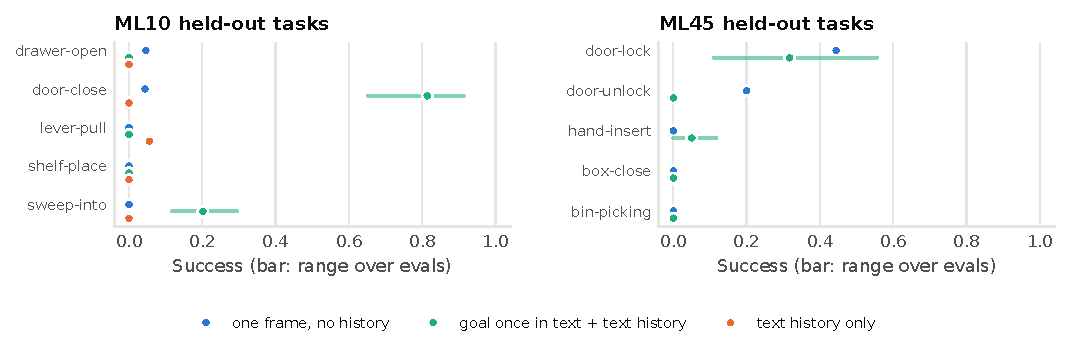
\includegraphics[width=\linewidth]{figures/goalhist.pdf}
\caption{Held-out tasks, per task: the one-frame 400-step clones (one per-task eval, 20 episodes per task) against
clones that see the goal once in text and keep the text history (mean of the seven evals at RL steps 0--60, 20
episodes per task each; the bar spans them). ML10 also: the history without the goal in text, and policies that state
the goal themselves (goal estimate cloned from the true offset; evals so far).}
\label{fig:goalhist}
\end{figure}

\textbf{ML10: held-out 0.02 $\to$ 0.22.} Over seven evals (steps 0--60, 100 held-out episodes each) the held-out tasks
average 0.22 (0.19--0.25), against 0.02 for the one-frame clone: door-close 0.81 (0.04) and sweep-into 0.20 (0). The
clone's training tasks rise too, 0.70 against 0.61 on the same 200-episode eval, mostly on point-goal tasks (reach 0.30
$\to$ 1.00, door-open 0.24 $\to$ 0.48, window-open 0.82 $\to$ 1.00; push falls 0.94 $\to$ 0.61). RL at lr 2e-6 keeps both
level (training tasks 0.71 over the seven evals).

\textbf{How the policy uses it: dead reckoning.} The transcripts show the clone replying with the \emph{remaining}
offset each turn (dx 75.2, then 65.5, 56.1, 46.8, \dots, cm), subtracting the moves it has made; the 10 cm cap turns that
into steady progress. On door-close, moving the hand to the goal point pushes the door shut, so ``go to the stated
point'', learned from the training tasks, solves it. On lever-pull the policy also reaches the goal, but without hooking
the lever. The transfer is real but specific: it helps held-out tasks whose goal point is where the hand should go.

\textbf{ML45: no held-out gain.} The clone fits the training tasks better, 0.61 against 0.49 (same 270-episode eval;
0.67 after 60 RL steps), but transfers less: held-out 0.03 at the clone, rising with RL to 0.12 at step 60, 0.07 over the
seven evals, against the one-frame clone's 0.12 (door-lock 0.32 vs 0.44, door-unlock 0 vs 0.20). ML45's held-out gains
came from look-alike tasks, and the stated goal did not add to them.

\textbf{The stated goal does the work, not the history.} The same text history without the goal in text
(\code{prompt\_style=compact\_rel}, \code{max\_frames=null}, \code{max\_images=1}): ML10's clone scores 0.66 on the
training tasks (reach 0.85) and 0.01 on the held-out tasks, door-close 0/20 (0.74 and 0.01 after 60 RL steps).
Remembering its own moves helps the policy fit (0.61 $\to$ 0.66) but transfers nothing; transfer appears only when it
is told where the goal is.

\textbf{Can the policy find the goal itself? Only on the training tasks.} Here nothing about the goal is given
(\code{prompt\_style=compact\_rel\_locate}): each reply first states where the goal is relative to the hand, then the move
(\code{Goal: dx=+12.0, dy=-3.5, dz=+4.0. \{"dx": 3.0, \dots\}}), and cloning trains the stated goal on the true offset,
from the simulator state the scripted experts already use. On the training tasks the estimate is good: median error
3.4\,cm with one frame, 1.3\,cm with the text history. On the held-out tasks it is 31 / 26\,cm off (door-close 70 / 85,
drawer-open 26 / 28, lever-pull 29 / 26, shelf-place 20 / 8, sweep-into 24 / 6), and held-out success stays at 0.01--0.03
(training tasks 0.65 / 0.69; RL at lr 2e-6 changes neither through step 20). The held-out estimates jump from turn to
turn and resemble the training tasks' offsets: the policy learned where each training task's goal usually is, not how to
find a goal marker. Here that is easy: within a training task the goal varies by only 0--7\,cm per axis (standard
deviation over variations, often 0 vertically), so the task nearly determines the offset. The markers do show these
held-out goals: each sits at the goal, and door-close's 71\,cm offset is real (its hand starts 50\,cm left of the door).

\takeaway{Stating the goal once and keeping the text history raised ML10's held-out tasks from 0.02 to 0.22, almost all
on door-close, by turning ``move the hand to the goal'' into a skill that carries over. The history alone does not
transfer: the gain is the stated goal, which is more precise than the marker (it includes depth). Asked to state the
goal themselves, clones find training-task goals within 1--3\,cm and miss held-out ones by 26--31\,cm: with ten tasks
whose goals barely move, goal finding is memorized per task. Even with the goal given, ML45's held-out tasks did not
improve, so for most held-out tasks the missing piece is the motion, not the goal.}

\section{What would improve held-out tasks?}
\label{sec:whatnext}
Held-out tasks are zero-shot: the policy never trains on them. Everything so far points to one diagnosis.

\textbf{Imitation learns to replay, task by task.}
\begin{itemize}
\item \emph{Motions.} The clones follow the instruction (the swap test) but fail tasks whose motion no training task
  showed; ML45 transfers only to look-alikes (door-lock, door-unlock).
\item \emph{Perception.} Asked to state the goal, the clones memorize each task's goal: 1--3\,cm off on training tasks,
  26--31\,cm on held-out ones (Section~\ref{sec:goalhist}).
\item \emph{Nothing we added changed it}: a larger model (9B), cloned rationales, the text history, RL from the clones
  (it refines what was cloned), REINFORCE++, and more training tasks (10 random tasks transfer as much as 45).
\end{itemize}
This is the regime of $\pi_{0.5}$ in PEAR's comparison: fine-tuned on LIBERO demonstrations it scores 96.9\% on LIBERO
but 0.75\% on LIBERO-Pro's unseen tasks in training scenes, because it ``replays the motion it was shown''.

\textbf{What the mazes teach.} Procedural mazes transferred to new layouts, and push to new positions once cloned on
450 of them (0.28 $\to$ 0.69): within one task family, variety forces the policy to use the observation. Held-out
\emph{tasks} are new task classes, with no maze analogue. The maze lesson reaches them only through the training tasks'
own variety, e.g.\ goals that move far enough that they must be read from the image, and that can at most reach the
goal-given ceiling (ML10 0.22, ML45 no gain). A second maze lesson: RL from sparse success worked because the base
models sometimes succeeded. On Metaworld the 4B base scores $\approx$0, and RL alone finds only the easiest tasks
(Section~\ref{sec:rlonly}).

\textbf{Would more tasks fix it?} ML10 $\to$ ML45 raised held-out transfer from 0.02 to 0.12, all on look-alikes. If
transfer is replay of the nearest training motion, it grows with how well the training tasks cover the held-out
motions, not with their number, and Metaworld has no further tasks to add. Tested directly: clones on subsets of
ML45's training tasks (same 400 cloning steps), all evaluated on ML45's held-out tasks (Fig.~\ref{fig:ntasks}).
\emph{Ten random tasks transfer as much as all 45} (0.11 vs 0.12: door-lock 0.28, door-unlock 0.25), \emph{twenty
transfer less} (0.04; the twenty include the ten), and the ten tasks I chose as motion look-alikes (door-open, door-close,
dial-turn, handle and lever tasks, pick tasks) transfer least (0.01). Transfer does not grow with the number of tasks and
is not predicted by which tasks look similar to us; within 0--0.12 it moves with which motions happen to dominate the
clone (with 20 episodes per task, differences below $\sim$0.06 overall are noise). More Metaworld tasks will not fix
held-out tasks for a cloned policy.

\begin{figure}[h]
\centering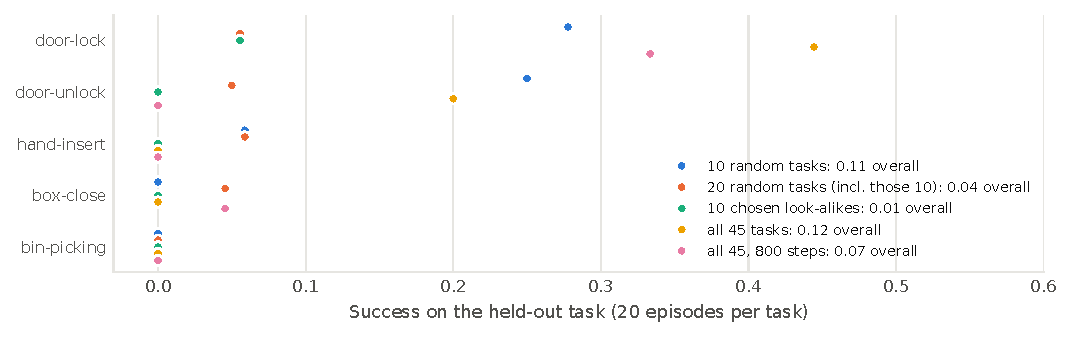
\includegraphics[width=\linewidth]{figures/ntasks.pdf}
\caption{ML45's held-out tasks for clones on 10 random, 20 random (a superset of the 10) and 10 chosen ML45 training
tasks (400 cloning steps each, eval right after cloning), and on all 45 (400 and 800 steps).}
\label{fig:ntasks}
\end{figure}

\textbf{Would another environment (LIBERO) help?} PEAR's numbers say the method, not the environment, made the
difference: on the same LIBERO-Pro unseen tasks, cloned $\pi_{0.5}$ gets 0.75\% and PEAR 57.4\%. PEAR is RL only (no
demonstrations) from a 27B reasoning model, with long reasoning before every move (at low reasoning effort its LIBERO
score falls from 74.4\% to 21.9\%) and every earlier round in context. LIBERO-Pro's unseen tasks also share scenes and
objects with training tasks, which makes them closer than Metaworld's new task classes. Our cloning recipe on LIBERO
would most likely reproduce $\pi_{0.5}$'s pattern; switching environments is worth it once a method transfers.

\textbf{So: the reasoning route, with a base model that can reason.} Our only transfer without a stated goal came from
RL with reasoning (held-out door-close 0.52 at step 30, lost by step 40), on a 4B model whose native thinking does not
finish (87\% invalid replies). Running: the same RL-only reasoning with Qwen3.5-9B, and zero-shot probes of Qwen3.5-9B,
27B and 35B-A3B with native thinking on ML10's training and held-out tasks, to find a base model that acts sensibly and
finishes its reasoning, the starting point RL from scratch needs.

\textbf{First probe: our axis description blocks reasoning.} Qwen3.5-9B with native thinking (8192 tokens, temperature
0.6), zero-shot on ML10: 0.02 on the training tasks and 0 on the held-out ones, with 77\% of replies never finishing.
The reasoning was not about the task: 93\% of replies re-read our description of the axes (``+dx moves the hand to the
right, +dy to the left, both slightly away from the camera'', true for the diagonal corner view), 88\% called it
confusing or contradictory and 64\% a typo, and the average reply mentions ``dy'' 143 times. Clones never noticed:
they learn the mapping from examples. For a policy that reasons, the frame has to be plain, so moves can now be given
in a camera-aligned frame (\code{env\_kwargs.action\_frame=camera}: +dx right in the image, +dy away from the camera, +dz
up, computed from the camera's pose).

\textbf{In the camera frame the reasoning is about the task, but the base models still solve only drawer-close.}
Unfinished replies fall from 77\% to 34--42\% (9B) and 30--35\% (35B-A3B), and talk of confusion from about 90\% to 30\%
of replies. Success, zero-shot with thinking: 9B 0.06 on the training tasks (drawer-close 1.00, every other task 0),
35B-A3B 0.04 (drawer-close 0.67); both 0 on every held-out task. The next obstacle shows in the transcripts: on reach the
35B sees ``a red ball floating in the air'', which is the goal marker, takes it for an unrelated object and tries to grasp
the objects on the table. Neither our prompt nor Metaworld's instructions (``Move the hand to the goal position'') say
what marks the goal. A short note on the scene's conventions (\code{env\_kwargs.scene\_notes=true}: the gripper, the
goal spheres, how grasping works; the same information as the image, stated) is next, with thinking and with short
reasoning (256 tokens, the length RL can afford: thinking at up to 8192 tokens per move, 15 moves, 128 episodes, is
up to 15M generated tokens per RL step).

\textbf{With the scene explained, the reasoning is right but the moves are not.} Zero-shot, camera frame, scene notes,
one frame in context: with short reasoning (256 tokens, greedy) Qwen3.5-4B, 9B and 27B solve nothing but drawer-close
(0 / 0.02 / 0 on the training tasks), 35B-A3B 0.06 (drawer-close 1.00) with 0.02 on the held-out tasks (door-close
0.08). With long thinking (no notes) the 27B scores 0.06 and solves held-out drawer-open in 0.10 of episodes, which
no clone does. The 35B's sentences are now correct (``the green sphere (goal) is to the left of the puck''), but it moves
1--2\,cm at a time (``slightly to the left''), re-plans from scratch every turn (open, close, open: with one frame in
context it cannot see that it just did that) and, on reach, still goes for the puck. What a reasoning agent lacks
here is what PEAR's agent has: the earlier turns in context, and positions in numbers.

\textbf{With the history and the object's position, an untrained 9B transfers as well as our best clone.} The text
history alone does not help (9B 0.00 / 0.00, 35B-A3B 0.02 / 0.00 on training / held-out tasks). Adding, every turn,
where the task's object is relative to the hand (\code{env\_kwargs.object\_text=true}: Metaworld's observation has the
object's position for every task, and the ML benchmarks hide only the goal, so this is not privileged) gives the base
Qwen3.5-9B \textbf{0.18 on ML10's held-out tasks} (door-close 0.69) and 0.10 on the training tasks, with no training at
all. With the goal offset at the first turn as well: 9B 0.18 (door-close 0.54, lever-pull 0.11, sweep-into 0.12) and
35B-A3B 0.22 (door-close 0.77, lever-pull 0.11). Lever-pull and sweep-into are held-out tasks no clone has solved. The
transcripts read like a sensible agent: ``the gripper is open and to the left of the door handle; move toward the
handle'', with moves sized from the numbers (dx $+$25, then $+$14, $+$8), and on lever-pull ``grasp the handle, then
lift'', failing on the grasp. (50 episodes per set, about 10 per held-out task: per-task numbers are rough.) Held-out
is not special for an untrained model, so the question becomes whether RL on the training tasks raises the held-out
tasks with them, as in PEAR, or specializes as our clones did. Running: RL from the base 9B with short reasoning,
text history and the object's position, on ML10 (with and without the goal offset) and on ML45. Their step-0 evals
(the untrained model, 100 episodes per set) confirm the probes: ML10 0.05 / 0.12 (door-close 0.52), with the goal offset
0.09 / 0.11, and on ML45 \textbf{0.20 on the 45 training tasks and 0.15 on the held-out ones} (door-lock 0.44,
door-unlock 0.35), above our best ML45 clone (0.12) without any training.

\begin{table}[h]
\centering\small
\begin{tabular}{llcccccrrr}
\toprule
Model & Reasoning & Axes & Notes & History & Object & Goal & Training & Held-out & Unfinished \\
\midrule
9B & thinking & world &  &  &  &  & 0.02 & 0.00 & 0.77 \\
9B & thinking & camera &  &  &  &  & 0.06 & 0.00 & 0.42 \\
27B & thinking & camera &  &  &  &  & 0.06 & 0.02 & 0.36 \\
35B-A3B & thinking & camera &  &  &  &  & 0.04 & 0.00 & 0.35 \\
4B & short & camera & \textbullet &  &  &  & 0.00 & 0.00 & 0.00 \\
9B & short & camera & \textbullet &  &  &  & 0.02 & 0.00 & 0.00 \\
27B & short & camera & \textbullet &  &  &  & 0.00 & 0.00 & 0.00 \\
35B-A3B & short & camera & \textbullet &  &  &  & 0.06 & 0.02 & 0.02 \\
9B & short & camera & \textbullet & \textbullet &  &  & 0.00 & 0.00 & 0.00 \\
35B-A3B & short & camera & \textbullet & \textbullet &  &  & 0.02 & 0.00 & 0.00 \\
9B & short & camera & \textbullet & \textbullet & \textbullet &  & 0.10 & 0.18 & 0.00 \\
35B-A3B & short & camera & \textbullet & \textbullet & \textbullet &  & 0.06 & 0.04 & 0.00 \\
9B & short & camera & \textbullet & \textbullet & \textbullet & \textbullet & 0.10 & 0.18 & 0.00 \\
35B-A3B & short & camera & \textbullet & \textbullet & \textbullet & \textbullet & 0.08 & 0.22 & 0.02 \\
\bottomrule
\end{tabular}

\caption{Zero-shot probes of base models on ML10 (no training; 50 training-task and 50 held-out episodes each).
Reasoning: native thinking (8192 tokens, temperature 0.6) or a short reason before each move (256 tokens, greedy).
Axes: Metaworld's world axes or camera-aligned. Notes: the scene's conventions stated. History: earlier turns' text in
context. Object / goal: the task's object (every turn) / the goal (first turn) relative to the hand. Unfinished: replies
without a readable move on training tasks.}
\label{tab:probes}
\end{table}

\textbf{Model size alone does not help RL with short reasoning.} The 4B run repeated with Qwen3.5-9B (world frame, same
settings): at step 40 it has learned drawer-close (0.64) and nothing else (training tasks 0.04; the 4B had 0.10, with
some reach and window-open), and 0 on every held-out task.

\section{Methodology lessons}
\label{sec:noise}
\begin{itemize}
\item \textbf{Greedy evals are not reproducible.} vLLM's greedy decoding is not bit-exact across servers and batch
  compositions; near-ties in a digit flip, and over 15 turns the episode diverges. The same push clone scored 0.12, 0.16
  and 0.31 on held-out positions in three runs. With 32 episodes the 95\% interval at $p=0.25$ is about $\pm0.15$. Pool
  evals, show intervals, and lean on the 128 training rollouts per step.
\item \textbf{Three cheap diagnostics} explained most failures: the step-1 mean log-prob (no exploration $\to$ no signal),
  its drift during training (sharpening toward a deterministic policy), and reply length (shrinking replies preceded every
  small-model collapse). The trainer-vs-vLLM log-prob gap on the same tokens checks that training is on-policy.
\item \textbf{Run the expert through your own interface first.} It measures the ceiling of the protocol, and here it
  exposed the controller gain.
\item \textbf{Check splits for leakage} before adding data: Metaworld ML1's seed 1 training split is seed 0's test split.
\end{itemize}

%=====================================================================================================================
\section{What did not work, in one table}
{\centering\small
\begin{tabular}{>{\raggedright\arraybackslash}p{4.4cm}>{\raggedright\arraybackslash}p{3.6cm}>{\raggedright\arraybackslash}p{7.2cm}}
\toprule
Approach & Result & Why \\
\midrule
Token-mean loss on SmolVLM2-2.2B & collapse in 5 updates & long failed episodes dominate the tokens; updates net negative \\
Lower lr / warmup / format penalty & only delayed the collapse & they do not change the token weighting \\
RL alone, less exploratory models & 0 on reach & near-deterministic sampling: groups tie, no signal \\
RL alone on push (any start) & 0 & never samples the multi-phase motion \\
Dense-reward preference on push & RL undid the clone & local optimum: grip the puck and hold still \\
DAgger with scripted experts & clone 0.20 $\to$ 0.00 & threshold experts give visually identical states opposite labels \\
DART with 2 cm noise & worse clone & the noisy expert itself succeeds only 0.20 \\
More cloning on 50 push positions & held-out stays 0.28 & memorizes the training configurations (450 positions: 0.69) \\
RL from the memorized clone & held-out flat or down & sharpens the memorized behaviour \\
RL (lr 1e-5) from good clones & push held-out falls, ML10 level & sharpens on its own samples \\
ML10 held-out tasks, one frame & $\approx$0 everywhere & too few training tasks for task transfer \\
Text history without the goal & ML10 held-out 0.01 & memory alone does not find held-out goals \\
More (or similar) training tasks & ML45 held-out 0.11 / 0.04 / 0.12 with 10 / 20 / 45 tasks & not count-driven; 10 chosen look-alikes 0.01 \\
Policy states the goal itself (cloned) & ML10 held-out 0.01--0.03 & estimates memorized per task: 26--31\,cm off on held-out tasks \\
RL alone on ML10, 32 groups/step & 0.08--0.10 (steps 40--170) & same plateau as 16 groups: multi-phase motions never sampled \\
\bottomrule
\end{tabular}\par}

\section{Open questions and next steps}
\begin{itemize}
\item Training tasks: scaling the cloning gets ML45 to 0.73 (expert ceiling 0.82); ML10 saturates at 0.67--0.69 (expert
  0.91). Which tasks stay unsolved, and why? Held-out tasks: ML45 transfers a little, best at 400 cloning steps (0.12), less at 800
  (0.056); RL does not raise it.
\item Held-out tasks are evaluated zero-shot throughout, by choice: no adaptation phase (no RL or cloning on the held-out
  tasks), although the ML10/ML45 meta-RL protocol would allow one. Held-out motions have to transfer from the training
  tasks.
\item Reach plateaus at 0.6--0.8 on held-out positions while training positions reach 0.9--1.0: more positions (as for push)
  should narrow that gap.
\item Held-out tasks: see Section~\ref{sec:whatnext} for the diagnosis and the experiments running.
\item The goal-in-text gain (Section~\ref{sec:goalhist}) is the stated goal, not the history, and a policy trained to state
  the goal itself memorizes it per task. Goal finding that transfers would need training tasks whose goals move a lot
  (or many more tasks); even then, the goal-given ceiling is small (ML10 0.22, mostly door-close; ML45 no gain).
\item A larger eval (128+ episodes) or pooled evals would make step-to-step comparisons meaningful.
\end{itemize}

\appendix
\section{Runs used}
\label{app:runs}
Every curve and number above comes from these wandb runs (entity \code{tri}; \code{maze/} = project
\code{vlm-rl-pointmaze}, \code{mw/} = project \code{vlm-rl-metaworld}). The scripted-expert success rates (Fig.~\ref{fig:expert}) were measured separately by driving
\code{metaworld.policies} through the environment's text protocol (\code{vlmrl.envs.metaworld.oracle\_action}).

{\small\begin{longtable}{@{}llll@{}}
\toprule
Key & Run & wandb group & Model \\
\midrule
\endhead
\texttt{pg\_qwen2b} & \texttt{7273b286} & \texttt{maze/procgen-fft-v2-diag} & Qwen3-VL-2B \\
\texttt{pg\_minicpm} & \texttt{23055312} & \texttt{maze/procgen-fft-v3-exact} & MiniCPM-V-4.6 \\
\texttt{pg\_gemma} & \texttt{3e97482a} & \texttt{maze/procgen-fft-v2} & gemma-4-E2B \\
\texttt{pg\_smol22\_traj} & \texttt{e320a919} & \texttt{maze/procgen-fft-v3-exact-trajmean} & SmolVLM2-2.2B \\
\texttt{fx\_500m\_umaze} & \texttt{da33c51b} & \texttt{maze/smolvlm2-fixed-maze-v1} & SmolVLM2-500M \\
\texttt{fx\_500m\_medium} & \texttt{86e6b888} & \texttt{maze/smolvlm2-fixed-maze-v1} & SmolVLM2-500M \\
\texttt{fx\_22\_tok\_umaze} & \texttt{39d8029d} & \texttt{maze/smolvlm2-fixed-maze-v1} & SmolVLM2-2.2B \\
\texttt{fx\_22\_tok\_medium} & \texttt{e532811d} & \texttt{maze/smolvlm2-fixed-maze-v1} & SmolVLM2-2.2B \\
\texttt{fx\_22\_traj\_umaze} & \texttt{73150cd4} & \texttt{maze/smolvlm2-fixed-maze-v1-trajmean} & SmolVLM2-2.2B \\
\texttt{fx\_22\_traj\_medium} & \texttt{1eb55355} & \texttt{maze/smolvlm2-fixed-maze-v1-trajmean} & SmolVLM2-2.2B \\
\texttt{fx\_22\_trajkl\_umaze} & \texttt{f118986b} & \texttt{maze/smolvlm2-fixed-maze-v1-trajmean-kl} & SmolVLM2-2.2B \\
\texttt{fx\_22\_trajkl\_medium} & \texttt{077253d8} & \texttt{maze/smolvlm2-fixed-maze-v1-trajmean-kl} & SmolVLM2-2.2B \\
\texttt{r\_q35} & \texttt{f1bc2e04} & \texttt{mw/metaworld-q35-v3-lr1e-5} & Qwen3.5-4B \\
\texttt{r\_q3vl4b\_bc} & \texttt{726835b5} & \texttt{mw/metaworld-bc2-q3vl4b-reach} & Qwen3-VL-4B \\
\texttt{r\_gemma\_bc} & \texttt{d092d258} & \texttt{mw/metaworld-bc2-gemma4-reach} & gemma-4-E2B \\
\texttt{r\_q3vl2b\_t16} & \texttt{69f4f4fc} & \texttt{mw/metaworld-reach-q3vl2b-t16} & Qwen3-VL-2B \\
\texttt{r\_gemma\_t16} & \texttt{8cea117b} & \texttt{mw/metaworld-reach-gemma4-t16} & gemma-4-E2B \\
\texttt{r\_q3vl4b\_t12} & \texttt{b39008c2} & \texttt{mw/metaworld-reach-q3vl4b} & Qwen3-VL-4B \\
\texttt{r\_q3vl2b\_t12} & \texttt{448f683a} & \texttt{mw/metaworld-reach-q3vl2b} & Qwen3-VL-2B \\
\texttt{r\_gemma\_t12} & \texttt{d6e2f340} & \texttt{mw/metaworld-reach-gemma4} & gemma-4-E2B \\
\texttt{r\_q3vl4b\_t16} & \texttt{7bf0dea1} & \texttt{mw/metaworld-reach-q3vl4b-t16} & Qwen3-VL-4B \\
\texttt{r\_q3vl4b\_t20} & \texttt{ccb99dd9} & \texttt{mw/metaworld-reach-q3vl4b-t20} & Qwen3-VL-4B \\
\texttt{p\_rl\_from\_reach} & \texttt{4a80c58d} & \texttt{mw/metaworld-q35-v4-push-from-reach} & Qwen3.5-4B \\
\texttt{p\_rl\_from\_reach\_t16} & \texttt{47188e19} & \texttt{mw/metaworld-q35-v4-push-from-reach-t16} & Qwen3.5-4B \\
\texttt{p1\_bc\_prefmw} & \texttt{a6c19ea2} & \texttt{mw/metaworld-bc2-q35-push} & Qwen3.5-4B \\
\texttt{p1\_bc\_prefobj} & \texttt{ed31ad85} & \texttt{mw/metaworld-bc3-q35-push} & Qwen3.5-4B \\
\texttt{p1\_q3vl4b\_bc} & \texttt{a1aeb101} & \texttt{mw/metaworld-bc3-q3vl4b-push} & Qwen3-VL-4B \\
\texttt{p1\_dagger} & \texttt{b8487691} & \texttt{mw/metaworld-bc4-q35-push-dagger} & Qwen3.5-4B \\
\texttt{p1\_dart1} & \texttt{51e3aa75} & \texttt{mw/metaworld-bc5-q35-push-dart1} & Qwen3.5-4B \\
\texttt{p1\_dart2} & \texttt{7fecc5dd} & \texttt{mw/metaworld-bc5-q35-push-dart2} & Qwen3.5-4B \\
\texttt{p1\_dart1\_t08} & \texttt{ca608d8c} & \texttt{mw/metaworld-bc6-q35-push-dart1-t08} & Qwen3.5-4B \\
\texttt{p1\_dart1\_t10} & \texttt{ed962f90} & \texttt{mw/metaworld-bc6-q35-push-dart1-t10} & Qwen3.5-4B \\
\texttt{p5\_bc30} & \texttt{223fd849} & \texttt{mw/metaworld-g05-q35-push} & Qwen3.5-4B \\
\texttt{p5\_dart30} & \texttt{65571a85} & \texttt{mw/metaworld-g05-q35-push-dart} & Qwen3.5-4B \\
\texttt{p5\_q3vl4b\_bc30} & \texttt{00238be4} & \texttt{mw/metaworld-g05-q3vl4b-push} & Qwen3-VL-4B \\
\texttt{p5\_bc100} & \texttt{a80a57d1} & \texttt{mw/metaworld-g05-q35-push-bc100} & Qwen3.5-4B \\
\texttt{p5\_q3vl4b\_bc100} & \texttt{782211cf} & \texttt{mw/metaworld-g05-q3vl4b-push-bc100} & Qwen3-VL-4B \\
\texttt{p5\_seeds10} & \texttt{9f6f5f04} & \texttt{mw/metaworld-g05-q35-push-seeds10} & Qwen3.5-4B \\
\texttt{m\_rl} & \texttt{147bb6b9} & \texttt{mw/metaworld-q35-v3-lr1e-5} & Qwen3.5-4B \\
\texttt{m\_from\_reach} & \texttt{3e049c7c} & \texttt{mw/metaworld-q35-v4-ml10-from-reach} & Qwen3.5-4B \\
\texttt{m1\_bc\_prefmw} & \texttt{ddd405a9} & \texttt{mw/metaworld-bc2-q35-ml10} & Qwen3.5-4B \\
\texttt{m1\_bc\_prefobj} & \texttt{2e436798} & \texttt{mw/metaworld-bc3-q35-ml10} & Qwen3.5-4B \\
\texttt{m1\_dagger} & \texttt{16467d2b} & \texttt{mw/metaworld-bc4-q35-ml10-dagger} & Qwen3.5-4B \\
\texttt{m1\_dart} & \texttt{c7413f19} & \texttt{mw/metaworld-bc5-q35-ml10-dart1} & Qwen3.5-4B \\
\texttt{m5\_bc30} & \texttt{337e1e20} & \texttt{mw/metaworld-g05-q35-ml10} & Qwen3.5-4B \\
\texttt{m5\_bc100} & \texttt{351850a4} & \texttt{mw/metaworld-g05-q35-ml10-bc100} & Qwen3.5-4B \\
\texttt{m5\_bc200} & \texttt{971c5b8e} & \texttt{mw/metaworld-g05-q35-ml10-bc200} & Qwen3.5-4B \\
\texttt{rc\_q35\_ml10} & \texttt{2fc1890d} & \texttt{mw/metaworld-recipe-q35-ml10} & Qwen3.5-4B \\
\texttt{rc\_q35\_ml45} & \texttt{39e1bda8} & \texttt{mw/metaworld-recipe-q35-ml45} & Qwen3.5-4B \\
\texttt{rc\_q3vl4b\_ml45} & \texttt{373b6478} & \texttt{mw/metaworld-recipe-q3vl4b-ml45} & Qwen3-VL-4B \\
\texttt{rc\_q35\_ml10\_rl2e6} & \texttt{f38dfa51} & \texttt{mw/metaworld-recipe-q35-ml10-rl2e-6} & Qwen3.5-4B \\
\texttt{rc\_q35\_ml45\_rl2e6} & \texttt{546903df} & \texttt{mw/metaworld-recipe-q35-ml45-rl2e-6} & Qwen3.5-4B \\
\texttt{rc\_q35\_ml45\_bc800} & \texttt{531a7bba} & \texttt{mw/metaworld-recipe-q35-ml45-bc800} & Qwen3.5-4B \\
\texttt{rc\_q35\_ml10\_bc400} & \texttt{00fb15f0} & \texttt{mw/metaworld-recipe-q35-ml10-bc400} & Qwen3.5-4B \\
\texttt{rc\_q35\_ml10\_bc800} & \texttt{ba1a1e50} & \texttt{mw/metaworld-recipe-q35-ml10-bc800} & Qwen3.5-4B \\
\texttt{rl\_push\_lr} & \texttt{55a5f8d6} & \texttt{mw/metaworld-rlfix-push450-lr2e-6} & Qwen3.5-4B \\
\texttt{rl\_push\_pos} & \texttt{4eb5ea24} & \texttt{mw/metaworld-rlfix-push450-posadv} & Qwen3.5-4B \\
\texttt{rl\_ml10\_lr} & \texttt{b4d50e68} & \texttt{mw/metaworld-rlfix-ml10-lr2e-6} & Qwen3.5-4B \\
\texttt{rl\_ml10\_pos} & \texttt{a92665ad} & \texttt{mw/metaworld-rlfix-ml10-posadv} & Qwen3.5-4B \\
\bottomrule
\end{longtable}
}

\section{Settings}
\begin{itemize}
\item \textbf{Metaworld:} 16 groups $\times$ 8 rollouts per step, 15 turns, replies of at most 128 tokens, temperature 1.2
  (1.0 for RL from push/ML10 clones), \code{traj\_mean}, no KL. Qwen3.5-4B: LoRA rank 64 on the language model's MLPs,
  lr 1e-5. Qwen3-VL-4B: LoRA rank 64, lr 1e-5. Qwen3-VL-2B: full fine-tuning, lr 2e-6. Gemma 4 E2B: full fine-tuning with
  the vision tower frozen, lr 1e-6. Behaviour cloning: 64 expert episodes per step (successful ones only), lr 5e-5 for
  LoRA, 1e-5 for Gemma.
\item \textbf{Mazes:} 32 groups $\times$ 16 rollouts, temperature 1.0, sparse success reward; procedural mazes 40 steps,
  fixed mazes 100 steps.
\item \textbf{Rebuild:} \code{uv run scripts/make\_results\_pdf.py -{}-fetch} (needs wandb credentials) refreshes
  \code{reports/data/runs.json}; without \code{-{}-fetch} the figures, tables and PDF are rebuilt from the cache.
\end{itemize}

\end{document}
